\documentclass[twoside]{book}

% Packages required by doxygen
\usepackage{fixltx2e}
\usepackage{calc}
\usepackage{doxygen}
\usepackage[export]{adjustbox} % also loads graphicx
\usepackage{graphicx}
\usepackage[utf8]{inputenc}
\usepackage{makeidx}
\usepackage{multicol}
\usepackage{multirow}
\PassOptionsToPackage{warn}{textcomp}
\usepackage{textcomp}
\usepackage[nointegrals]{wasysym}
\usepackage[table]{xcolor}

% Font selection
\usepackage[T1]{fontenc}
\usepackage[scaled=.90]{helvet}
\usepackage{courier}
\usepackage{amssymb}
\usepackage{sectsty}
\renewcommand{\familydefault}{\sfdefault}
\allsectionsfont{%
  \fontseries{bc}\selectfont%
  \color{darkgray}%
}
\renewcommand{\DoxyLabelFont}{%
  \fontseries{bc}\selectfont%
  \color{darkgray}%
}
\newcommand{\+}{\discretionary{\mbox{\scriptsize$\hookleftarrow$}}{}{}}

% Page & text layout
\usepackage{geometry}
\geometry{%
  a4paper,%
  top=2.5cm,%
  bottom=2.5cm,%
  left=2.5cm,%
  right=2.5cm%
}
\tolerance=750
\hfuzz=15pt
\hbadness=750
\setlength{\emergencystretch}{15pt}
\setlength{\parindent}{0cm}
\setlength{\parskip}{3ex plus 2ex minus 2ex}
\makeatletter
\renewcommand{\paragraph}{%
  \@startsection{paragraph}{4}{0ex}{-1.0ex}{1.0ex}{%
    \normalfont\normalsize\bfseries\SS@parafont%
  }%
}
\renewcommand{\subparagraph}{%
  \@startsection{subparagraph}{5}{0ex}{-1.0ex}{1.0ex}{%
    \normalfont\normalsize\bfseries\SS@subparafont%
  }%
}
\makeatother

% Headers & footers
\usepackage{fancyhdr}
\pagestyle{fancyplain}
\fancyhead[LE]{\fancyplain{}{\bfseries\thepage}}
\fancyhead[CE]{\fancyplain{}{}}
\fancyhead[RE]{\fancyplain{}{\bfseries\leftmark}}
\fancyhead[LO]{\fancyplain{}{\bfseries\rightmark}}
\fancyhead[CO]{\fancyplain{}{}}
\fancyhead[RO]{\fancyplain{}{\bfseries\thepage}}
\fancyfoot[LE]{\fancyplain{}{}}
\fancyfoot[CE]{\fancyplain{}{}}
\fancyfoot[RE]{\fancyplain{}{\bfseries\scriptsize Generated by Doxygen }}
\fancyfoot[LO]{\fancyplain{}{\bfseries\scriptsize Generated by Doxygen }}
\fancyfoot[CO]{\fancyplain{}{}}
\fancyfoot[RO]{\fancyplain{}{}}
\renewcommand{\footrulewidth}{0.4pt}
\renewcommand{\chaptermark}[1]{%
  \markboth{#1}{}%
}
\renewcommand{\sectionmark}[1]{%
  \markright{\thesection\ #1}%
}

% Indices & bibliography
\usepackage{natbib}
\usepackage[titles]{tocloft}
\setcounter{tocdepth}{3}
\setcounter{secnumdepth}{5}
\makeindex

% Hyperlinks (required, but should be loaded last)
\usepackage{ifpdf}
\ifpdf
  \usepackage[pdftex,pagebackref=true]{hyperref}
\else
  \usepackage[ps2pdf,pagebackref=true]{hyperref}
\fi
\hypersetup{%
  colorlinks=true,%
  linkcolor=blue,%
  citecolor=blue,%
  unicode%
}

% Custom commands
\newcommand{\clearemptydoublepage}{%
  \newpage{\pagestyle{empty}\cleardoublepage}%
}

\usepackage{caption}
\captionsetup{labelsep=space,justification=centering,font={bf},singlelinecheck=off,skip=4pt,position=top}

%===== C O N T E N T S =====

\begin{document}

% Titlepage & ToC
\hypersetup{pageanchor=false,
             bookmarksnumbered=true,
             pdfencoding=unicode
            }
\pagenumbering{alph}
\begin{titlepage}
\vspace*{7cm}
\begin{center}%
{\Large M\+OS }\\
\vspace*{1cm}
{\large Generated by Doxygen 1.8.13}\\
\end{center}
\end{titlepage}
\clearemptydoublepage
\pagenumbering{roman}
\tableofcontents
\clearemptydoublepage
\pagenumbering{arabic}
\hypersetup{pageanchor=true}

%--- Begin generated contents ---
\chapter{mos}
\label{md_README}
\Hypertarget{md_README}
M\+OS, or Maintainable R\+T\+OS, is a simple and lightweight R\+T\+OS microkernel for the A\+RM Cortex M series that supports basic threading and I\+PC primitives.

It is a work in progress and is intended for \char`\"{}fun personal projects.\char`\"{}

M\+OS was originally developed on a S\+T\+Microelectronics S\+T\+M32\+F4 Discovery and has been tested on the following boards\+:
\begin{DoxyItemize}
\item S\+T\+M32\+F767\+ZI Nucleo-\/144 (A\+RM Cortex M7)
\item S\+T\+M32\+L562 Discovery Kit (A\+RM Cortex M33)
\item S\+T\+M32\+F4 Discovery (A\+RM Cortex M4F)
\item S\+T\+M32\+G071\+RB Nucleo (A\+RM Cortex M0+)
\end{DoxyItemize}

Design Goals\+:
\begin{DoxyItemize}
\item R\+T\+OS\+: Hard priorities and bounded execution.
\item Short critical sections.
\item Simple configuration with low use of conditional compilation.
\item Tick reduction ({\itshape i.\+e.\+:} the so-\/called \char`\"{}tickless\char`\"{} operation).
\item Small code size ({\itshape e.\+g.\+:} mos/kernel$\ast$.c compiled size is $\sim$5\+KB).
\item Static kernel and (optionally) static application.
\item Easily customizable.
\item Provide example B\+S\+Ps and example applications.
\end{DoxyItemize}

Included Primitives\+:
\begin{DoxyItemize}
\item Recursive mutex with priority inheritance
\item Semaphores (counting / multi-\/bit binary)
\item Message queues (multi-\/priority)
\item Sys\+Tick-\/based timers
\end{DoxyItemize}

Included Optional Modules\+:
\begin{DoxyItemize}
\item Heap
\item Shared context (cooperative multitasking where clients share same thread and message queue, intended for small memory footprints)
\item Logging
\item Command shell
\item Test bench
\end{DoxyItemize}

Supported toolchains / architectures\+:
\begin{DoxyItemize}
\item G\+CC
\item A\+RM M0/\+M1/\+M0+ (Arch v6-\/M)
\item A\+RM M3/\+M4/\+M7 (Arch v7-\/M)
\item A\+RM M4\+F/\+M7F (Arch v7-\/M with hardware floating point using lazy stacking)
\item A\+RM M23/\+M33/\+M55 (Arch v8-\/M) -\/ currently supporting a single security mode\+: secure or non-\/secure.
\item Trust\+Zone can be used with interrupts disabled.
\end{DoxyItemize}

Future
\begin{DoxyItemize}
\item Better documentation...
\item Support Context switches in Trust\+Zone
\item C++ bindings
\end{DoxyItemize}

Features it probably W\+I\+LL N\+E\+V\+ER have\+:
\begin{DoxyItemize}
\item Full M\+PU support
\item Non-\/\+A\+RM architecture support
\item Non-\/\+G\+CC toolchain support 
\end{DoxyItemize}
\chapter{Class Index}
\section{Class List}
Here are the classes, structs, unions and interfaces with brief descriptions\+:\begin{DoxyCompactList}
\item\contentsline{section}{\hyperlink{structBlock}{Block} }{\pageref{structBlock}}{}
\item\contentsline{section}{\hyperlink{structLink}{Link} }{\pageref{structLink}}{}
\item\contentsline{section}{\hyperlink{structMosClient}{Mos\+Client} }{\pageref{structMosClient}}{}
\item\contentsline{section}{\hyperlink{structMosContext}{Mos\+Context} }{\pageref{structMosContext}}{}
\item\contentsline{section}{\hyperlink{structMosContextMessage}{Mos\+Context\+Message} }{\pageref{structMosContextMessage}}{}
\item\contentsline{section}{\hyperlink{structMosContextTimer}{Mos\+Context\+Timer} }{\pageref{structMosContextTimer}}{}
\item\contentsline{section}{\hyperlink{structMosFIFO32}{Mos\+F\+I\+F\+O32} }{\pageref{structMosFIFO32}}{}
\item\contentsline{section}{\hyperlink{structMosHeap}{Mos\+Heap} }{\pageref{structMosHeap}}{}
\item\contentsline{section}{\hyperlink{structMosLinkHet}{Mos\+Link\+Het} }{\pageref{structMosLinkHet}}{}
\item\contentsline{section}{\hyperlink{structMosList}{Mos\+List} }{\pageref{structMosList}}{}
\item\contentsline{section}{\hyperlink{structMosMutex}{Mos\+Mutex} }{\pageref{structMosMutex}}{}
\item\contentsline{section}{\hyperlink{structMosParams}{Mos\+Params} }{\pageref{structMosParams}}{}
\item\contentsline{section}{\hyperlink{structMosPool}{Mos\+Pool} }{\pageref{structMosPool}}{}
\item\contentsline{section}{\hyperlink{structMosQueue}{Mos\+Queue} }{\pageref{structMosQueue}}{}
\item\contentsline{section}{\hyperlink{structMosSem}{Mos\+Sem} }{\pageref{structMosSem}}{}
\item\contentsline{section}{\hyperlink{structMosShell}{Mos\+Shell} }{\pageref{structMosShell}}{}
\item\contentsline{section}{\hyperlink{structMosShellCommand}{Mos\+Shell\+Command} }{\pageref{structMosShellCommand}}{}
\item\contentsline{section}{\hyperlink{structMosThread}{Mos\+Thread} }{\pageref{structMosThread}}{}
\item\contentsline{section}{\hyperlink{structMosTimer}{Mos\+Timer} }{\pageref{structMosTimer}}{}
\item\contentsline{section}{\hyperlink{structSlab}{Slab} }{\pageref{structSlab}}{}
\item\contentsline{section}{\hyperlink{structStackFrame}{Stack\+Frame} }{\pageref{structStackFrame}}{}
\item\contentsline{section}{\hyperlink{structThread}{Thread} }{\pageref{structThread}}{}
\item\contentsline{section}{\hyperlink{unionTicker}{Ticker} }{\pageref{unionTicker}}{}
\end{DoxyCompactList}

\chapter{File Index}
\section{File List}
Here is a list of all documented files with brief descriptions\+:\begin{DoxyCompactList}
\item\contentsline{section}{\hyperlink{mos__config_8h}{mos\+\_\+config.\+h} \\*M\+OS Configuration File }{\pageref{mos__config_8h}}{}
\item\contentsline{section}{bsp/{\bfseries hal\+\_\+tb.\+h} }{\pageref{hal__tb_8h}}{}
\item\contentsline{section}{mos/{\bfseries arch.\+h} }{\pageref{arch_8h}}{}
\item\contentsline{section}{mos/\hyperlink{context_8h}{context.\+h} \\*Shared Contexts }{\pageref{context_8h}}{}
\item\contentsline{section}{mos/{\bfseries defs.\+h} }{\pageref{defs_8h}}{}
\item\contentsline{section}{mos/{\bfseries fifo.\+h} }{\pageref{fifo_8h}}{}
\item\contentsline{section}{mos/{\bfseries format\+\_\+string.\+h} }{\pageref{format__string_8h}}{}
\item\contentsline{section}{mos/{\bfseries hal.\+h} }{\pageref{hal_8h}}{}
\item\contentsline{section}{mos/\hyperlink{heap_8h}{heap.\+h} \\*M\+OS Heap }{\pageref{heap_8h}}{}
\item\contentsline{section}{mos/\hyperlink{kernel_8h}{kernel.\+h} \\*M\+OS Microkernel }{\pageref{kernel_8h}}{}
\item\contentsline{section}{mos/\hyperlink{list_8h}{list.\+h} \\*Doubly-\/\+Linked Circular Lists }{\pageref{list_8h}}{}
\item\contentsline{section}{mos/\hyperlink{queue_8h}{queue.\+h} \\*M\+OS Message Queues }{\pageref{queue_8h}}{}
\item\contentsline{section}{mos/{\bfseries shell.\+h} }{\pageref{shell_8h}}{}
\item\contentsline{section}{mos/{\bfseries slab.\+h} }{\pageref{slab_8h}}{}
\item\contentsline{section}{mos/{\bfseries thread\+\_\+heap.\+h} }{\pageref{thread__heap_8h}}{}
\item\contentsline{section}{mos/{\bfseries trace.\+h} }{\pageref{trace_8h}}{}
\end{DoxyCompactList}

\chapter{Class Documentation}
\hypertarget{structBlock}{}\section{Block Struct Reference}
\label{structBlock}\index{Block@{Block}}


Collaboration diagram for Block\+:\nopagebreak
\begin{figure}[H]
\begin{center}
\leavevmode
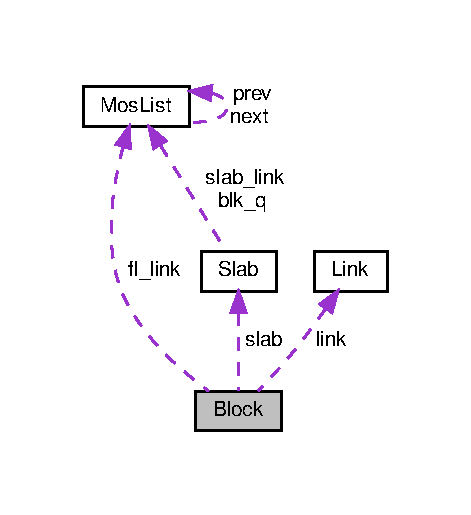
\includegraphics[width=226pt]{structBlock__coll__graph}
\end{center}
\end{figure}
\subsection*{Public Attributes}
\begin{DoxyCompactItemize}
\item 
\mbox{\Hypertarget{structBlock_a9ac7db4278f6f2be4940e4c8ab54babc}\label{structBlock_a9ac7db4278f6f2be4940e4c8ab54babc}} 
\hyperlink{structLink}{Link} {\bfseries link}
\item 
\mbox{\Hypertarget{structBlock_abd410ea4590f9f56115513a10591ba88}\label{structBlock_abd410ea4590f9f56115513a10591ba88}} 
\begin{tabbing}
xx\=xx\=xx\=xx\=xx\=xx\=xx\=xx\=xx\=\kill
union \{\\
\>\hyperlink{structMosList}{MosLink} {\bfseries fl\_link}\\
\>u8 {\bfseries payload} \mbox{[}0\mbox{]}\\
\}; \\

\end{tabbing}\item 
\mbox{\Hypertarget{structBlock_a1df2961842ddce4cf14a113b3b73f15d}\label{structBlock_a1df2961842ddce4cf14a113b3b73f15d}} 
\hyperlink{structSlab}{Slab} $\ast$ {\bfseries slab}
\item 
\mbox{\Hypertarget{structBlock_a706059cece3f83de8fde1340632aa5eb}\label{structBlock_a706059cece3f83de8fde1340632aa5eb}} 
\begin{tabbing}
xx\=xx\=xx\=xx\=xx\=xx\=xx\=xx\=xx\=\kill
union \{\\
\>\hyperlink{structMosList}{MosLink} {\bfseries fl\_link}\\
\>u8 {\bfseries payload} \mbox{[}0\mbox{]}\\
\}; \\

\end{tabbing}\end{DoxyCompactItemize}


The documentation for this struct was generated from the following files\+:\begin{DoxyCompactItemize}
\item 
mos/heap.\+c\item 
mos/slab.\+c\end{DoxyCompactItemize}

\hypertarget{structLink}{}\section{Link Struct Reference}
\label{structLink}\index{Link@{Link}}
\subsection*{Public Attributes}
\begin{DoxyCompactItemize}
\item 
\mbox{\Hypertarget{structLink_a696c5493f016c6b4486c0ba00c9375fc}\label{structLink_a696c5493f016c6b4486c0ba00c9375fc}} 
u32 {\bfseries canary}
\item 
\mbox{\Hypertarget{structLink_a36f0a757a9435573d7dc282a6287266a}\label{structLink_a36f0a757a9435573d7dc282a6287266a}} 
u32 {\bfseries size\+\_\+p}
\item 
\mbox{\Hypertarget{structLink_a785d9cfe1769e87e5e0b7ce365c73975}\label{structLink_a785d9cfe1769e87e5e0b7ce365c73975}} 
u32 {\bfseries size}
\end{DoxyCompactItemize}


The documentation for this struct was generated from the following file\+:\begin{DoxyCompactItemize}
\item 
mos/heap.\+c\end{DoxyCompactItemize}

\hypertarget{structMosClient}{}\section{Mos\+Client Struct Reference}
\label{structMosClient}\index{Mos\+Client@{Mos\+Client}}


Collaboration diagram for Mos\+Client\+:\nopagebreak
\begin{figure}[H]
\begin{center}
\leavevmode
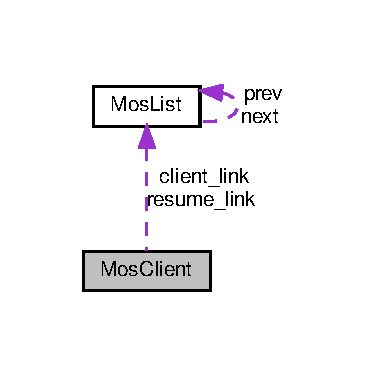
\includegraphics[width=176pt]{structMosClient__coll__graph}
\end{center}
\end{figure}
\subsection*{Public Attributes}
\begin{DoxyCompactItemize}
\item 
\mbox{\Hypertarget{structMosClient_afded4ff09a6d3a3d583cfa9e6ec85819}\label{structMosClient_afded4ff09a6d3a3d583cfa9e6ec85819}} 
Mos\+Client\+Handler $\ast$ {\bfseries handler}
\item 
\mbox{\Hypertarget{structMosClient_acd4c3f64b0550d3c7af5ecb37adcbe66}\label{structMosClient_acd4c3f64b0550d3c7af5ecb37adcbe66}} 
void $\ast$ {\bfseries priv\+\_\+data}
\item 
\mbox{\Hypertarget{structMosClient_a254ff0a6149f4e4548d75dde37f2db1c}\label{structMosClient_a254ff0a6149f4e4548d75dde37f2db1c}} 
\hyperlink{structMosList}{Mos\+Link} {\bfseries client\+\_\+link}
\item 
\mbox{\Hypertarget{structMosClient_a227da9bb9f58de9673cfb34126f190e9}\label{structMosClient_a227da9bb9f58de9673cfb34126f190e9}} 
\hyperlink{structMosList}{Mos\+Link} {\bfseries resume\+\_\+link}
\item 
\mbox{\Hypertarget{structMosClient_a7c79c3eb94a4b5e855791dafd9426b71}\label{structMosClient_a7c79c3eb94a4b5e855791dafd9426b71}} 
bool {\bfseries completed}
\end{DoxyCompactItemize}


The documentation for this struct was generated from the following file\+:\begin{DoxyCompactItemize}
\item 
mos/\hyperlink{context_8h}{context.\+h}\end{DoxyCompactItemize}

\hypertarget{structMosContext}{}\section{Mos\+Context Struct Reference}
\label{structMosContext}\index{Mos\+Context@{Mos\+Context}}


Collaboration diagram for Mos\+Context\+:\nopagebreak
\begin{figure}[H]
\begin{center}
\leavevmode
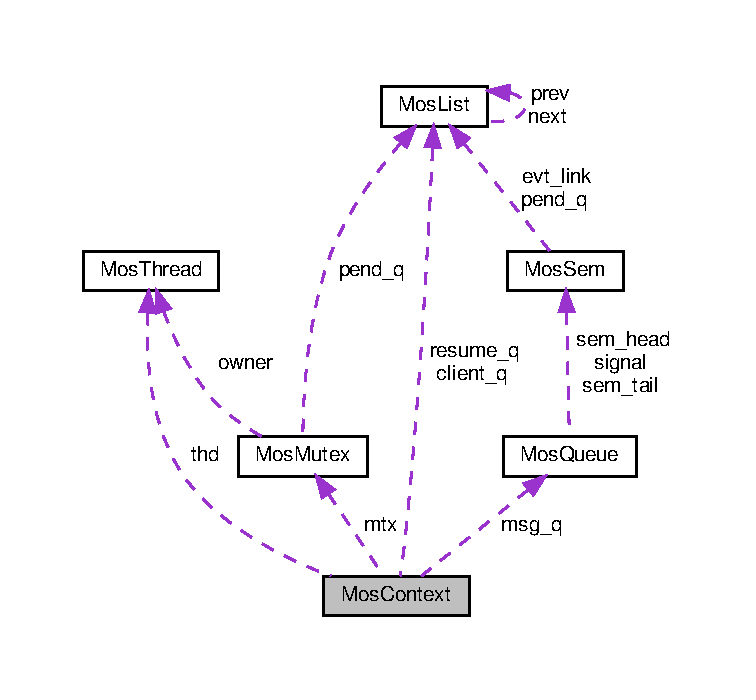
\includegraphics[width=350pt]{structMosContext__coll__graph}
\end{center}
\end{figure}
\subsection*{Public Attributes}
\begin{DoxyCompactItemize}
\item 
\mbox{\Hypertarget{structMosContext_ab7a3499d1074e84cbbacd1d40ce41b3c}\label{structMosContext_ab7a3499d1074e84cbbacd1d40ce41b3c}} 
\hyperlink{structMosMutex}{Mos\+Mutex} {\bfseries mtx}
\item 
\mbox{\Hypertarget{structMosContext_a00fc0de27a8c397adee827e24c952a1b}\label{structMosContext_a00fc0de27a8c397adee827e24c952a1b}} 
\hyperlink{structMosQueue}{Mos\+Queue} {\bfseries msg\+\_\+q}
\item 
\mbox{\Hypertarget{structMosContext_a50bb20493f573489758cb3863b81a7d7}\label{structMosContext_a50bb20493f573489758cb3863b81a7d7}} 
\hyperlink{structMosList}{Mos\+List} {\bfseries client\+\_\+q}
\item 
\mbox{\Hypertarget{structMosContext_a5631d32d11740ac71d1545d93cb0a35d}\label{structMosContext_a5631d32d11740ac71d1545d93cb0a35d}} 
\hyperlink{structMosList}{Mos\+List} {\bfseries resume\+\_\+q}
\item 
\mbox{\Hypertarget{structMosContext_a0377077c08a9eeb45ad7279ea5753b72}\label{structMosContext_a0377077c08a9eeb45ad7279ea5753b72}} 
\hyperlink{structMosThread}{Mos\+Thread} {\bfseries thd}
\end{DoxyCompactItemize}


The documentation for this struct was generated from the following file\+:\begin{DoxyCompactItemize}
\item 
mos/\hyperlink{context_8h}{context.\+h}\end{DoxyCompactItemize}

\hypertarget{structMosContextMessage}{}\section{Mos\+Context\+Message Struct Reference}
\label{structMosContextMessage}\index{Mos\+Context\+Message@{Mos\+Context\+Message}}


Collaboration diagram for Mos\+Context\+Message\+:\nopagebreak
\begin{figure}[H]
\begin{center}
\leavevmode
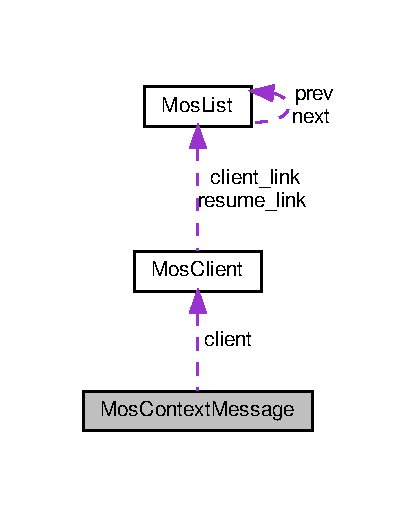
\includegraphics[width=201pt]{structMosContextMessage__coll__graph}
\end{center}
\end{figure}
\subsection*{Public Attributes}
\begin{DoxyCompactItemize}
\item 
\mbox{\Hypertarget{structMosContextMessage_a453c6a2a36b77d43426ee02407283ac0}\label{structMosContextMessage_a453c6a2a36b77d43426ee02407283ac0}} 
struct \hyperlink{structMosClient}{Mos\+Client} $\ast$ {\bfseries client}
\item 
\mbox{\Hypertarget{structMosContextMessage_ae762d897f62444833dfc88cbae2345c1}\label{structMosContextMessage_ae762d897f62444833dfc88cbae2345c1}} 
Mos\+Context\+Message\+ID {\bfseries id}
\item 
\mbox{\Hypertarget{structMosContextMessage_abea2109a6afbf96cd8df72f6e9445a4a}\label{structMosContextMessage_abea2109a6afbf96cd8df72f6e9445a4a}} 
void $\ast$ {\bfseries data}
\end{DoxyCompactItemize}


The documentation for this struct was generated from the following file\+:\begin{DoxyCompactItemize}
\item 
mos/\hyperlink{context_8h}{context.\+h}\end{DoxyCompactItemize}

\hypertarget{structMosContextTimer}{}\section{Mos\+Context\+Timer Struct Reference}
\label{structMosContextTimer}\index{Mos\+Context\+Timer@{Mos\+Context\+Timer}}


Collaboration diagram for Mos\+Context\+Timer\+:\nopagebreak
\begin{figure}[H]
\begin{center}
\leavevmode
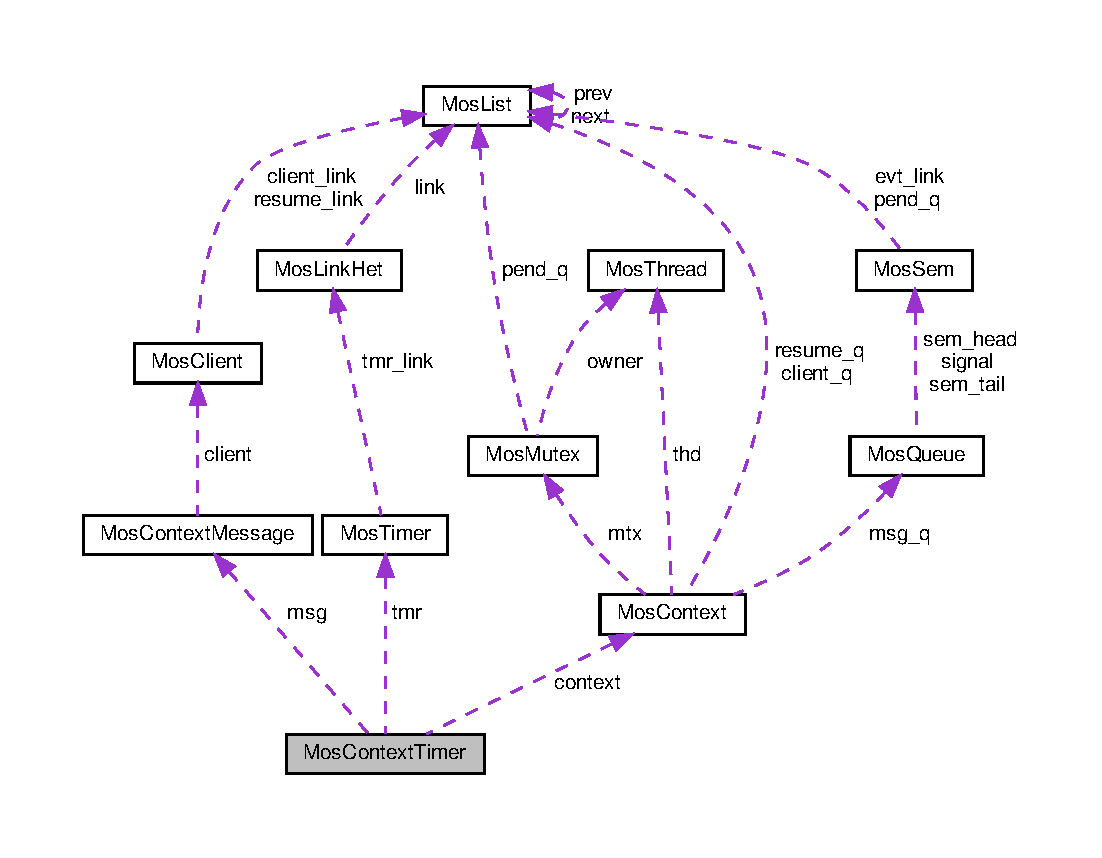
\includegraphics[width=350pt]{structMosContextTimer__coll__graph}
\end{center}
\end{figure}
\subsection*{Public Attributes}
\begin{DoxyCompactItemize}
\item 
\mbox{\Hypertarget{structMosContextTimer_a3bd17a42e0b1dfe08327b6271bef0bc1}\label{structMosContextTimer_a3bd17a42e0b1dfe08327b6271bef0bc1}} 
\hyperlink{structMosTimer}{Mos\+Timer} {\bfseries tmr}
\item 
\mbox{\Hypertarget{structMosContextTimer_a6c89658eb791d4bbc186f30711f1db04}\label{structMosContextTimer_a6c89658eb791d4bbc186f30711f1db04}} 
\hyperlink{structMosContext}{Mos\+Context} $\ast$ {\bfseries context}
\item 
\mbox{\Hypertarget{structMosContextTimer_a7619e23e27b9693685e190b5cae76d97}\label{structMosContextTimer_a7619e23e27b9693685e190b5cae76d97}} 
\hyperlink{structMosContextMessage}{Mos\+Context\+Message} {\bfseries msg}
\end{DoxyCompactItemize}


The documentation for this struct was generated from the following file\+:\begin{DoxyCompactItemize}
\item 
mos/\hyperlink{context_8h}{context.\+h}\end{DoxyCompactItemize}

\hypertarget{structMosFIFO32}{}\section{Mos\+F\+I\+F\+O32 Struct Reference}
\label{structMosFIFO32}\index{Mos\+F\+I\+F\+O32@{Mos\+F\+I\+F\+O32}}
\subsection*{Public Attributes}
\begin{DoxyCompactItemize}
\item 
\mbox{\Hypertarget{structMosFIFO32_a5eb1d98c5f8c776f57ad6778e59f3190}\label{structMosFIFO32_a5eb1d98c5f8c776f57ad6778e59f3190}} 
volatile u32 $\ast$ {\bfseries buf}
\item 
\mbox{\Hypertarget{structMosFIFO32_abce3395b3a68379262ab2d2b9c7663e7}\label{structMosFIFO32_abce3395b3a68379262ab2d2b9c7663e7}} 
u32 {\bfseries len}
\item 
\mbox{\Hypertarget{structMosFIFO32_a7c3a0c1ee1957dce9f90805d4e05587d}\label{structMosFIFO32_a7c3a0c1ee1957dce9f90805d4e05587d}} 
volatile u32 {\bfseries tail}
\item 
\mbox{\Hypertarget{structMosFIFO32_a03eefc208e06b1f30aba58e127c2e623}\label{structMosFIFO32_a03eefc208e06b1f30aba58e127c2e623}} 
volatile u32 {\bfseries head}
\end{DoxyCompactItemize}


The documentation for this struct was generated from the following file\+:\begin{DoxyCompactItemize}
\item 
mos/fifo.\+h\end{DoxyCompactItemize}

\hypertarget{structMosHeap}{}\section{Mos\+Heap Struct Reference}
\label{structMosHeap}\index{Mos\+Heap@{Mos\+Heap}}


Collaboration diagram for Mos\+Heap\+:\nopagebreak
\begin{figure}[H]
\begin{center}
\leavevmode
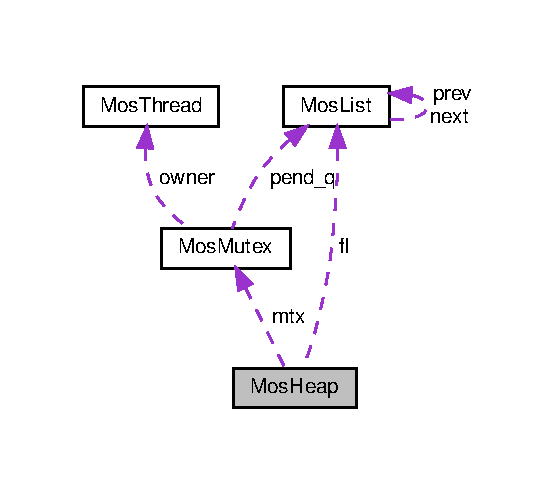
\includegraphics[width=267pt]{structMosHeap__coll__graph}
\end{center}
\end{figure}
\subsection*{Public Attributes}
\begin{DoxyCompactItemize}
\item 
\mbox{\Hypertarget{structMosHeap_ac1f21f9b3444ba6e39a35941fef2b8d8}\label{structMosHeap_ac1f21f9b3444ba6e39a35941fef2b8d8}} 
\hyperlink{structMosMutex}{Mos\+Mutex} {\bfseries mtx}
\item 
\mbox{\Hypertarget{structMosHeap_a330bbbbbb97880f9108fe2655c035802}\label{structMosHeap_a330bbbbbb97880f9108fe2655c035802}} 
\hyperlink{structMosList}{Mos\+List} {\bfseries fl}
\item 
\mbox{\Hypertarget{structMosHeap_a9cb5599f50592171ab7a5f3d2fed25a9}\label{structMosHeap_a9cb5599f50592171ab7a5f3d2fed25a9}} 
u32 {\bfseries bytes\+\_\+free}
\item 
\mbox{\Hypertarget{structMosHeap_a5455d71a4efaf4ac5db03c861077b911}\label{structMosHeap_a5455d71a4efaf4ac5db03c861077b911}} 
u32 {\bfseries min\+\_\+bytes\+\_\+free}
\item 
\mbox{\Hypertarget{structMosHeap_a1fcf6dc27b69893dfb6fb6a50afbea23}\label{structMosHeap_a1fcf6dc27b69893dfb6fb6a50afbea23}} 
u16 {\bfseries align\+\_\+mask}
\item 
\mbox{\Hypertarget{structMosHeap_a61e4c7b2ef32a8e1b53668228e67e7a1}\label{structMosHeap_a61e4c7b2ef32a8e1b53668228e67e7a1}} 
u16 {\bfseries fl\+\_\+block\+\_\+cnt}
\item 
\mbox{\Hypertarget{structMosHeap_a6752200325f092909228c3e0f001f64d}\label{structMosHeap_a6752200325f092909228c3e0f001f64d}} 
u16 {\bfseries min\+\_\+block\+\_\+size}
\end{DoxyCompactItemize}


The documentation for this struct was generated from the following file\+:\begin{DoxyCompactItemize}
\item 
mos/\hyperlink{heap_8h}{heap.\+h}\end{DoxyCompactItemize}

\hypertarget{structMosLinkHet}{}\section{Mos\+Link\+Het Struct Reference}
\label{structMosLinkHet}\index{Mos\+Link\+Het@{Mos\+Link\+Het}}


Collaboration diagram for Mos\+Link\+Het\+:\nopagebreak
\begin{figure}[H]
\begin{center}
\leavevmode
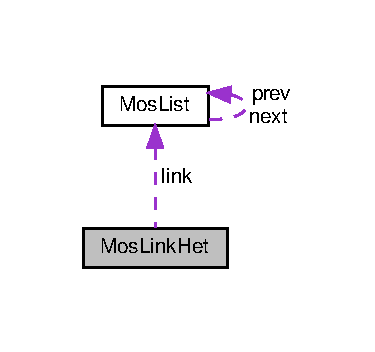
\includegraphics[width=180pt]{structMosLinkHet__coll__graph}
\end{center}
\end{figure}
\subsection*{Public Attributes}
\begin{DoxyCompactItemize}
\item 
\mbox{\Hypertarget{structMosLinkHet_acb2e233a5da5848bd284575efd158f7a}\label{structMosLinkHet_acb2e233a5da5848bd284575efd158f7a}} 
\hyperlink{structMosList}{Mos\+Link} {\bfseries link}
\item 
\mbox{\Hypertarget{structMosLinkHet_a988c955f3fba0aef7681893203c37c0e}\label{structMosLinkHet_a988c955f3fba0aef7681893203c37c0e}} 
u32 {\bfseries type}
\end{DoxyCompactItemize}


The documentation for this struct was generated from the following file\+:\begin{DoxyCompactItemize}
\item 
mos/\hyperlink{list_8h}{list.\+h}\end{DoxyCompactItemize}

\hypertarget{structMosList}{}\section{Mos\+List Struct Reference}
\label{structMosList}\index{Mos\+List@{Mos\+List}}


Collaboration diagram for Mos\+List\+:\nopagebreak
\begin{figure}[H]
\begin{center}
\leavevmode
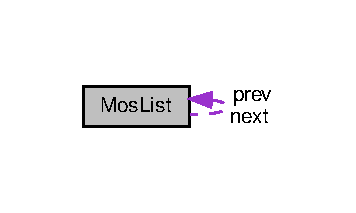
\includegraphics[width=171pt]{structMosList__coll__graph}
\end{center}
\end{figure}
\subsection*{Public Attributes}
\begin{DoxyCompactItemize}
\item 
\mbox{\Hypertarget{structMosList_acd83f0bcc6dcde24468183cf47b69f37}\label{structMosList_acd83f0bcc6dcde24468183cf47b69f37}} 
struct \hyperlink{structMosList}{Mos\+List} $\ast$ {\bfseries prev}
\item 
\mbox{\Hypertarget{structMosList_ab119e85d9884731d627fb11b1c1366bb}\label{structMosList_ab119e85d9884731d627fb11b1c1366bb}} 
struct \hyperlink{structMosList}{Mos\+List} $\ast$ {\bfseries next}
\end{DoxyCompactItemize}


The documentation for this struct was generated from the following file\+:\begin{DoxyCompactItemize}
\item 
mos/\hyperlink{list_8h}{list.\+h}\end{DoxyCompactItemize}

\hypertarget{structMosMutex}{}\section{Mos\+Mutex Struct Reference}
\label{structMosMutex}\index{Mos\+Mutex@{Mos\+Mutex}}


Collaboration diagram for Mos\+Mutex\+:\nopagebreak
\begin{figure}[H]
\begin{center}
\leavevmode
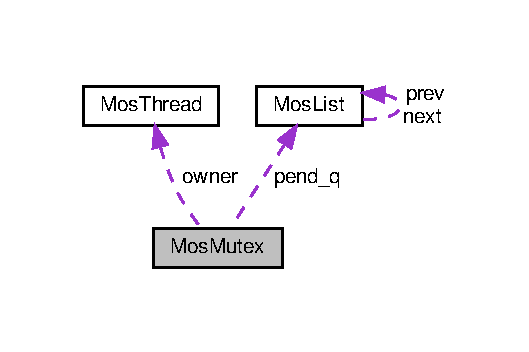
\includegraphics[width=254pt]{structMosMutex__coll__graph}
\end{center}
\end{figure}
\subsection*{Public Attributes}
\begin{DoxyCompactItemize}
\item 
\mbox{\Hypertarget{structMosMutex_a8eb138a40b29ebc00ddbf52701111403}\label{structMosMutex_a8eb138a40b29ebc00ddbf52701111403}} 
\hyperlink{structMosThread}{Mos\+Thread} $\ast$ {\bfseries owner}
\item 
\mbox{\Hypertarget{structMosMutex_ab0d64dea3a92b1035f39ecfd3f91c505}\label{structMosMutex_ab0d64dea3a92b1035f39ecfd3f91c505}} 
s32 {\bfseries depth}
\item 
\mbox{\Hypertarget{structMosMutex_abbd3035b55fb5212b2db25f8634870d1}\label{structMosMutex_abbd3035b55fb5212b2db25f8634870d1}} 
\hyperlink{structMosList}{Mos\+List} {\bfseries pend\+\_\+q}
\end{DoxyCompactItemize}


The documentation for this struct was generated from the following file\+:\begin{DoxyCompactItemize}
\item 
mos/\hyperlink{kernel_8h}{kernel.\+h}\end{DoxyCompactItemize}

\hypertarget{structMosParams}{}\section{Mos\+Params Struct Reference}
\label{structMosParams}\index{Mos\+Params@{Mos\+Params}}
\subsection*{Public Attributes}
\begin{DoxyCompactItemize}
\item 
\mbox{\Hypertarget{structMosParams_ae87ec56d27ce859148ad301afeea3390}\label{structMosParams_ae87ec56d27ce859148ad301afeea3390}} 
char $\ast$ {\bfseries version}
\item 
\mbox{\Hypertarget{structMosParams_a23d3ae62ad483de21b10bfbe8cbf9bab}\label{structMosParams_a23d3ae62ad483de21b10bfbe8cbf9bab}} 
Mos\+Thread\+Priority {\bfseries thread\+\_\+pri\+\_\+hi}
\item 
\mbox{\Hypertarget{structMosParams_a597614a4ad790e727c49b62acef610b9}\label{structMosParams_a597614a4ad790e727c49b62acef610b9}} 
Mos\+Thread\+Priority {\bfseries thread\+\_\+pri\+\_\+low}
\item 
\mbox{\Hypertarget{structMosParams_a41c13442ae606fe1c90cefb95b63f49c}\label{structMosParams_a41c13442ae606fe1c90cefb95b63f49c}} 
u32 {\bfseries int\+\_\+pri\+\_\+hi}
\item 
\mbox{\Hypertarget{structMosParams_af883999419b2bf5ecb3aeeb9e4506f3a}\label{structMosParams_af883999419b2bf5ecb3aeeb9e4506f3a}} 
u32 {\bfseries int\+\_\+pri\+\_\+low}
\item 
\mbox{\Hypertarget{structMosParams_a5a19cef0b7f76b3ab11034341bdc6f25}\label{structMosParams_a5a19cef0b7f76b3ab11034341bdc6f25}} 
u32 {\bfseries micro\+\_\+sec\+\_\+per\+\_\+tick}
\item 
\mbox{\Hypertarget{structMosParams_adcbc515ff9d63a33b61181168a7b52b2}\label{structMosParams_adcbc515ff9d63a33b61181168a7b52b2}} 
bool {\bfseries fp\+\_\+support\+\_\+en}
\end{DoxyCompactItemize}


The documentation for this struct was generated from the following file\+:\begin{DoxyCompactItemize}
\item 
mos/\hyperlink{kernel_8h}{kernel.\+h}\end{DoxyCompactItemize}

\hypertarget{structMosPool}{}\section{Mos\+Pool Struct Reference}
\label{structMosPool}\index{Mos\+Pool@{Mos\+Pool}}


Collaboration diagram for Mos\+Pool\+:\nopagebreak
\begin{figure}[H]
\begin{center}
\leavevmode
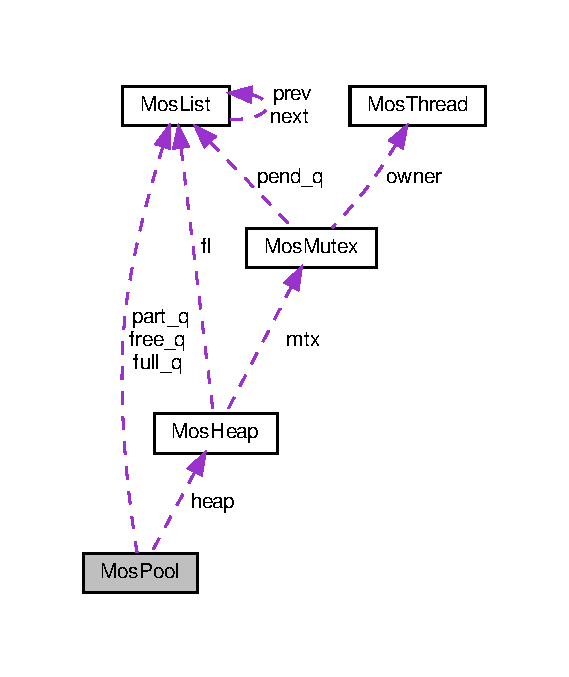
\includegraphics[width=273pt]{structMosPool__coll__graph}
\end{center}
\end{figure}
\subsection*{Public Attributes}
\begin{DoxyCompactItemize}
\item 
\mbox{\Hypertarget{structMosPool_a35db29268defbf37eda8afe57329c436}\label{structMosPool_a35db29268defbf37eda8afe57329c436}} 
\hyperlink{structMosList}{Mos\+List} {\bfseries part\+\_\+q}
\item 
\mbox{\Hypertarget{structMosPool_a52a4ef587c709e67243c2887437746f1}\label{structMosPool_a52a4ef587c709e67243c2887437746f1}} 
\hyperlink{structMosList}{Mos\+List} {\bfseries free\+\_\+q}
\item 
\mbox{\Hypertarget{structMosPool_a9c32ebd7f6832de03a02444f1025a394}\label{structMosPool_a9c32ebd7f6832de03a02444f1025a394}} 
\hyperlink{structMosList}{Mos\+List} {\bfseries full\+\_\+q}
\item 
\mbox{\Hypertarget{structMosPool_a1f328c700c820e2548dc31637b8477bd}\label{structMosPool_a1f328c700c820e2548dc31637b8477bd}} 
u32 {\bfseries avail\+\_\+blocks}
\item 
\mbox{\Hypertarget{structMosPool_ae8841c31465ac338c6092b8dca0ad6b3}\label{structMosPool_ae8841c31465ac338c6092b8dca0ad6b3}} 
\hyperlink{structMosHeap}{Mos\+Heap} $\ast$ {\bfseries heap}
\item 
\mbox{\Hypertarget{structMosPool_a0a5cec50ee6557c09685c76dd53f5db5}\label{structMosPool_a0a5cec50ee6557c09685c76dd53f5db5}} 
u32 {\bfseries block\+\_\+size}
\item 
\mbox{\Hypertarget{structMosPool_a257658d677e4c7f0040c536a1d89c10a}\label{structMosPool_a257658d677e4c7f0040c536a1d89c10a}} 
u32 {\bfseries slab\+\_\+size}
\item 
\mbox{\Hypertarget{structMosPool_ae3a072bf533eb64dcaaaa91f872dc7bb}\label{structMosPool_ae3a072bf533eb64dcaaaa91f872dc7bb}} 
u16 {\bfseries blocks\+\_\+per\+\_\+slab}
\item 
\mbox{\Hypertarget{structMosPool_a7def7c710420c4c753aa3b39bb30df77}\label{structMosPool_a7def7c710420c4c753aa3b39bb30df77}} 
u16 {\bfseries align\+\_\+mask}
\end{DoxyCompactItemize}


The documentation for this struct was generated from the following file\+:\begin{DoxyCompactItemize}
\item 
mos/slab.\+h\end{DoxyCompactItemize}

\hypertarget{structMosQueue}{}\section{Mos\+Queue Struct Reference}
\label{structMosQueue}\index{Mos\+Queue@{Mos\+Queue}}


Collaboration diagram for Mos\+Queue\+:\nopagebreak
\begin{figure}[H]
\begin{center}
\leavevmode
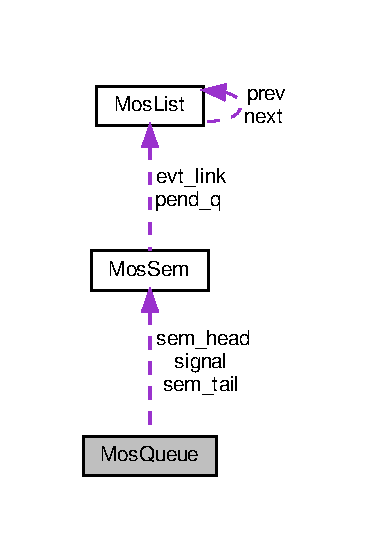
\includegraphics[width=178pt]{structMosQueue__coll__graph}
\end{center}
\end{figure}
\subsection*{Public Attributes}
\begin{DoxyCompactItemize}
\item 
\mbox{\Hypertarget{structMosQueue_a5335ad626efa53590597eeebd06693cb}\label{structMosQueue_a5335ad626efa53590597eeebd06693cb}} 
\hyperlink{structMosSem}{Mos\+Sem} {\bfseries sem\+\_\+tail}
\item 
\mbox{\Hypertarget{structMosQueue_a749f2e4ee9267fb52c4c6d9ebb213f87}\label{structMosQueue_a749f2e4ee9267fb52c4c6d9ebb213f87}} 
\hyperlink{structMosSem}{Mos\+Sem} {\bfseries sem\+\_\+head}
\item 
\mbox{\Hypertarget{structMosQueue_a2d916f7452ac6b3417107a3168b6601b}\label{structMosQueue_a2d916f7452ac6b3417107a3168b6601b}} 
u32 $\ast$ {\bfseries begin}
\item 
\mbox{\Hypertarget{structMosQueue_a6c5ec3ac8871d597e6e4b65768398781}\label{structMosQueue_a6c5ec3ac8871d597e6e4b65768398781}} 
u32 $\ast$ {\bfseries end}
\item 
\mbox{\Hypertarget{structMosQueue_a7c0a5b7c5060f6c4fe036ecf9180775e}\label{structMosQueue_a7c0a5b7c5060f6c4fe036ecf9180775e}} 
u32 $\ast$ {\bfseries tail}
\item 
\mbox{\Hypertarget{structMosQueue_aa722b5e1355f585373da2319f35b3911}\label{structMosQueue_aa722b5e1355f585373da2319f35b3911}} 
u32 $\ast$ {\bfseries head}
\item 
\mbox{\Hypertarget{structMosQueue_a33fd7b13bda2f199262b6dff3ad1158e}\label{structMosQueue_a33fd7b13bda2f199262b6dff3ad1158e}} 
u16 {\bfseries elm\+\_\+size}
\item 
\mbox{\Hypertarget{structMosQueue_aaedec79b2bf30f2122e717c968870776}\label{structMosQueue_aaedec79b2bf30f2122e717c968870776}} 
u16 {\bfseries channel}
\item 
\mbox{\Hypertarget{structMosQueue_ae7b9ae53f14ccb1987ac8be6bd3ef493}\label{structMosQueue_ae7b9ae53f14ccb1987ac8be6bd3ef493}} 
\hyperlink{structMosSem}{Mos\+Signal} $\ast$ {\bfseries signal}
\end{DoxyCompactItemize}


The documentation for this struct was generated from the following file\+:\begin{DoxyCompactItemize}
\item 
mos/\hyperlink{queue_8h}{queue.\+h}\end{DoxyCompactItemize}

\hypertarget{structMosSem}{}\section{Mos\+Sem Struct Reference}
\label{structMosSem}\index{Mos\+Sem@{Mos\+Sem}}


Collaboration diagram for Mos\+Sem\+:\nopagebreak
\begin{figure}[H]
\begin{center}
\leavevmode
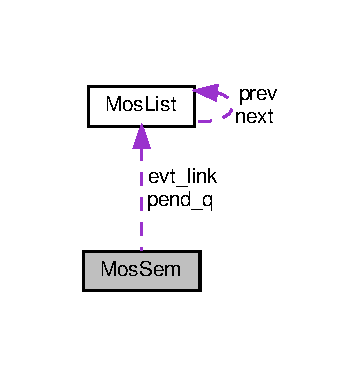
\includegraphics[width=174pt]{structMosSem__coll__graph}
\end{center}
\end{figure}
\subsection*{Public Attributes}
\begin{DoxyCompactItemize}
\item 
\mbox{\Hypertarget{structMosSem_a0085aae7b8bf75b68045b55d4a076f2b}\label{structMosSem_a0085aae7b8bf75b68045b55d4a076f2b}} 
u32 {\bfseries value}
\item 
\mbox{\Hypertarget{structMosSem_a0b6f281d95d804efcb503f7dba875dc3}\label{structMosSem_a0b6f281d95d804efcb503f7dba875dc3}} 
\hyperlink{structMosList}{Mos\+List} {\bfseries pend\+\_\+q}
\item 
\mbox{\Hypertarget{structMosSem_ac70d34b4f737bdc203d08af974a6903b}\label{structMosSem_ac70d34b4f737bdc203d08af974a6903b}} 
\hyperlink{structMosList}{Mos\+Link} {\bfseries evt\+\_\+link}
\end{DoxyCompactItemize}


The documentation for this struct was generated from the following file\+:\begin{DoxyCompactItemize}
\item 
mos/\hyperlink{kernel_8h}{kernel.\+h}\end{DoxyCompactItemize}

\hypertarget{structMosShell}{}\section{Mos\+Shell Struct Reference}
\label{structMosShell}\index{Mos\+Shell@{Mos\+Shell}}


Collaboration diagram for Mos\+Shell\+:\nopagebreak
\begin{figure}[H]
\begin{center}
\leavevmode
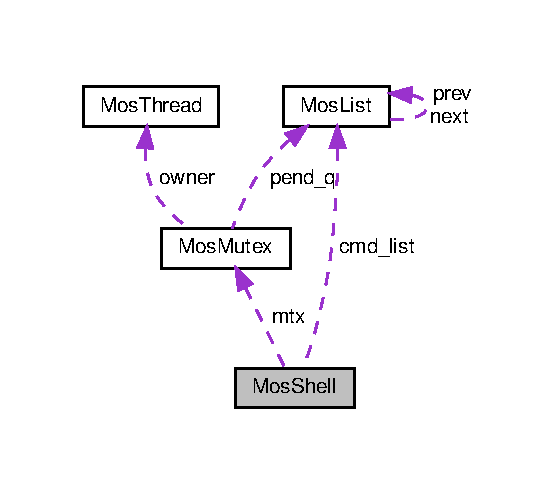
\includegraphics[width=267pt]{structMosShell__coll__graph}
\end{center}
\end{figure}
\subsection*{Public Attributes}
\begin{DoxyCompactItemize}
\item 
\mbox{\Hypertarget{structMosShell_ad385f409dd88d2c56c2cd7c863abfb18}\label{structMosShell_ad385f409dd88d2c56c2cd7c863abfb18}} 
\hyperlink{structMosMutex}{Mos\+Mutex} {\bfseries mtx}
\item 
\mbox{\Hypertarget{structMosShell_aceed2ca93728f39150d2820a3ac12917}\label{structMosShell_aceed2ca93728f39150d2820a3ac12917}} 
\hyperlink{structMosList}{Mos\+List} {\bfseries cmd\+\_\+list}
\item 
\mbox{\Hypertarget{structMosShell_a2322b8c62140118c8c5a1a85a010bc72}\label{structMosShell_a2322b8c62140118c8c5a1a85a010bc72}} 
void $\ast$ {\bfseries cmd\+\_\+buffer}
\item 
\mbox{\Hypertarget{structMosShell_a4e4095bd92770fa71bcb9e87f01b7ed5}\label{structMosShell_a4e4095bd92770fa71bcb9e87f01b7ed5}} 
u16 {\bfseries cmd\+\_\+buffer\+\_\+len}
\item 
\mbox{\Hypertarget{structMosShell_a35ea35dd5fffae9e530af96a0d7d8950}\label{structMosShell_a35ea35dd5fffae9e530af96a0d7d8950}} 
u16 {\bfseries max\+\_\+cmd\+\_\+line\+\_\+size}
\item 
\mbox{\Hypertarget{structMosShell_abdb8f7af3edea29d0f85c1d58112d15d}\label{structMosShell_abdb8f7af3edea29d0f85c1d58112d15d}} 
s16 {\bfseries cmd\+\_\+ix}
\item 
\mbox{\Hypertarget{structMosShell_aa654a50a58c707908f7ac9424f9d4844}\label{structMosShell_aa654a50a58c707908f7ac9424f9d4844}} 
s16 {\bfseries cmd\+\_\+max\+\_\+ix}
\item 
\mbox{\Hypertarget{structMosShell_ad6cd893593123bf76aa51863c28ae39a}\label{structMosShell_ad6cd893593123bf76aa51863c28ae39a}} 
s16 {\bfseries cmd\+\_\+history\+\_\+ix}
\end{DoxyCompactItemize}


The documentation for this struct was generated from the following file\+:\begin{DoxyCompactItemize}
\item 
mos/shell.\+h\end{DoxyCompactItemize}

\hypertarget{structMosShellCommand}{}\section{Mos\+Shell\+Command Struct Reference}
\label{structMosShellCommand}\index{Mos\+Shell\+Command@{Mos\+Shell\+Command}}


Collaboration diagram for Mos\+Shell\+Command\+:\nopagebreak
\begin{figure}[H]
\begin{center}
\leavevmode
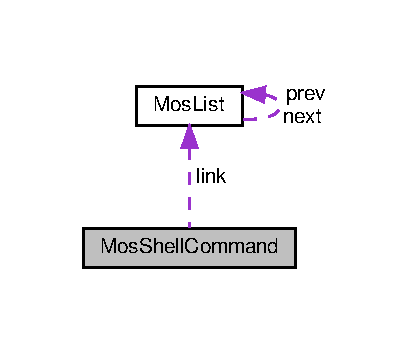
\includegraphics[width=197pt]{structMosShellCommand__coll__graph}
\end{center}
\end{figure}
\subsection*{Public Attributes}
\begin{DoxyCompactItemize}
\item 
\mbox{\Hypertarget{structMosShellCommand_a0bc9d73e1638c8d81b2f85cbeef4cdfb}\label{structMosShellCommand_a0bc9d73e1638c8d81b2f85cbeef4cdfb}} 
Mos\+Command\+Func $\ast$ {\bfseries func}
\item 
\mbox{\Hypertarget{structMosShellCommand_aed49fc90b1944413b60051b7a41b3b72}\label{structMosShellCommand_aed49fc90b1944413b60051b7a41b3b72}} 
char $\ast$ {\bfseries name}
\item 
\mbox{\Hypertarget{structMosShellCommand_a33df2ba720d7f1bb1b9be5bb76289eb4}\label{structMosShellCommand_a33df2ba720d7f1bb1b9be5bb76289eb4}} 
char $\ast$ {\bfseries desc}
\item 
\mbox{\Hypertarget{structMosShellCommand_a49c3168bcb084dac1d27fbc3989d75c3}\label{structMosShellCommand_a49c3168bcb084dac1d27fbc3989d75c3}} 
char $\ast$ {\bfseries usage}
\item 
\mbox{\Hypertarget{structMosShellCommand_a3f76a3694d6ac5a4db19aebce1fd9406}\label{structMosShellCommand_a3f76a3694d6ac5a4db19aebce1fd9406}} 
\hyperlink{structMosList}{Mos\+Link} {\bfseries link}
\end{DoxyCompactItemize}


The documentation for this struct was generated from the following file\+:\begin{DoxyCompactItemize}
\item 
mos/shell.\+h\end{DoxyCompactItemize}

\hypertarget{structMosThread}{}\section{Mos\+Thread Struct Reference}
\label{structMosThread}\index{Mos\+Thread@{Mos\+Thread}}
\subsection*{Public Attributes}
\begin{DoxyCompactItemize}
\item 
\mbox{\Hypertarget{structMosThread_a485202c0d8a788ffaf1c3daf046af79f}\label{structMosThread_a485202c0d8a788ffaf1c3daf046af79f}} 
u32 {\bfseries rsvd} \mbox{[}18\mbox{]}
\item 
\mbox{\Hypertarget{structMosThread_acf529fb4d8e9cc2aa7332cbc364e35e0}\label{structMosThread_acf529fb4d8e9cc2aa7332cbc364e35e0}} 
s32 {\bfseries ref\+\_\+cnt}
\end{DoxyCompactItemize}


The documentation for this struct was generated from the following file\+:\begin{DoxyCompactItemize}
\item 
mos/\hyperlink{kernel_8h}{kernel.\+h}\end{DoxyCompactItemize}

\hypertarget{structMosTimer}{}\section{Mos\+Timer Struct Reference}
\label{structMosTimer}\index{Mos\+Timer@{Mos\+Timer}}


Collaboration diagram for Mos\+Timer\+:\nopagebreak
\begin{figure}[H]
\begin{center}
\leavevmode
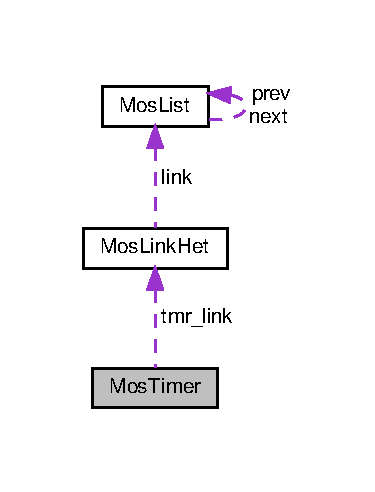
\includegraphics[width=180pt]{structMosTimer__coll__graph}
\end{center}
\end{figure}
\subsection*{Public Attributes}
\begin{DoxyCompactItemize}
\item 
\mbox{\Hypertarget{structMosTimer_aef14c6b3f240508770bf0fa2f5b34632}\label{structMosTimer_aef14c6b3f240508770bf0fa2f5b34632}} 
u32 {\bfseries ticks}
\item 
\mbox{\Hypertarget{structMosTimer_aecf6b6fc65c6799e07098d340e5d1708}\label{structMosTimer_aecf6b6fc65c6799e07098d340e5d1708}} 
u32 {\bfseries wake\+\_\+tick}
\item 
\mbox{\Hypertarget{structMosTimer_a877e79e2e2b0a641ff6cefdee403f4ab}\label{structMosTimer_a877e79e2e2b0a641ff6cefdee403f4ab}} 
\hyperlink{structMosLinkHet}{Mos\+Link\+Het} {\bfseries tmr\+\_\+link}
\item 
\mbox{\Hypertarget{structMosTimer_a60ff56f2039fda6e9695e74ed0224fcc}\label{structMosTimer_a60ff56f2039fda6e9695e74ed0224fcc}} 
Mos\+Timer\+Callback $\ast$ {\bfseries callback}
\item 
\mbox{\Hypertarget{structMosTimer_a50c5249cc6bb9d9270071646cbde1c5c}\label{structMosTimer_a50c5249cc6bb9d9270071646cbde1c5c}} 
void $\ast$ {\bfseries priv\+\_\+data}
\end{DoxyCompactItemize}


The documentation for this struct was generated from the following file\+:\begin{DoxyCompactItemize}
\item 
mos/\hyperlink{kernel_8h}{kernel.\+h}\end{DoxyCompactItemize}

\hypertarget{structSlab}{}\section{Slab Struct Reference}
\label{structSlab}\index{Slab@{Slab}}


Collaboration diagram for Slab\+:\nopagebreak
\begin{figure}[H]
\begin{center}
\leavevmode
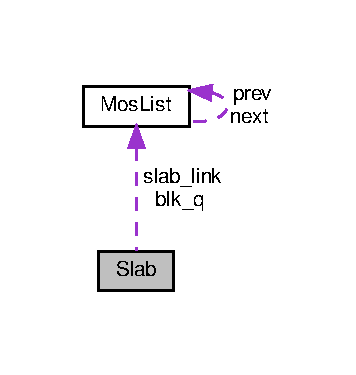
\includegraphics[width=171pt]{structSlab__coll__graph}
\end{center}
\end{figure}
\subsection*{Public Attributes}
\begin{DoxyCompactItemize}
\item 
\mbox{\Hypertarget{structSlab_ab8e004433995ac3d98fe46f0c26d0b15}\label{structSlab_ab8e004433995ac3d98fe46f0c26d0b15}} 
\hyperlink{structMosList}{Mos\+List} {\bfseries blk\+\_\+q}
\item 
\mbox{\Hypertarget{structSlab_a894e051abf1550b7cd2d5aba32eb6943}\label{structSlab_a894e051abf1550b7cd2d5aba32eb6943}} 
\hyperlink{structMosList}{Mos\+Link} {\bfseries slab\+\_\+link}
\item 
\mbox{\Hypertarget{structSlab_a2db39ad038c02dc4a7fd2c5bf96efec3}\label{structSlab_a2db39ad038c02dc4a7fd2c5bf96efec3}} 
u32 {\bfseries avail\+\_\+blocks}
\item 
\mbox{\Hypertarget{structSlab_a4d006626ec44ddaa310359b3597b8355}\label{structSlab_a4d006626ec44ddaa310359b3597b8355}} 
u8 {\bfseries align\+\_\+pad\+\_\+and\+\_\+blocks} \mbox{[}0\mbox{]}
\end{DoxyCompactItemize}


The documentation for this struct was generated from the following file\+:\begin{DoxyCompactItemize}
\item 
mos/slab.\+c\end{DoxyCompactItemize}

\hypertarget{structStackFrame}{}\section{Stack\+Frame Struct Reference}
\label{structStackFrame}\index{Stack\+Frame@{Stack\+Frame}}
\subsection*{Public Attributes}
\begin{DoxyCompactItemize}
\item 
\mbox{\Hypertarget{structStackFrame_aa0c7f76aaf7f2f1253ff4ca685382a3a}\label{structStackFrame_aa0c7f76aaf7f2f1253ff4ca685382a3a}} 
u32 {\bfseries S\+W\+S\+A\+VE} \mbox{[}8\mbox{]}
\item 
\mbox{\Hypertarget{structStackFrame_ab264ea9c3ded2a4ea46855db48ce2d86}\label{structStackFrame_ab264ea9c3ded2a4ea46855db48ce2d86}} 
u32 {\bfseries L\+R\+\_\+\+E\+X\+C\+\_\+\+R\+TN}
\item 
\mbox{\Hypertarget{structStackFrame_adc515b48af18333245add1f3d9fbdfce}\label{structStackFrame_adc515b48af18333245add1f3d9fbdfce}} 
u32 {\bfseries H\+W\+S\+A\+VE} \mbox{[}4\mbox{]}
\item 
\mbox{\Hypertarget{structStackFrame_ac4030991721c5f10e593ec97ead1525a}\label{structStackFrame_ac4030991721c5f10e593ec97ead1525a}} 
u32 {\bfseries R12}
\item 
\mbox{\Hypertarget{structStackFrame_a7b93475e91b65b664e4e409306f9f175}\label{structStackFrame_a7b93475e91b65b664e4e409306f9f175}} 
u32 {\bfseries LR}
\item 
\mbox{\Hypertarget{structStackFrame_aa617ff429f69a61a15ec6b88e565b631}\label{structStackFrame_aa617ff429f69a61a15ec6b88e565b631}} 
u32 {\bfseries PC}
\item 
\mbox{\Hypertarget{structStackFrame_ab81daac3bde3228aa4509380466f6749}\label{structStackFrame_ab81daac3bde3228aa4509380466f6749}} 
u32 {\bfseries P\+SR}
\end{DoxyCompactItemize}


The documentation for this struct was generated from the following file\+:\begin{DoxyCompactItemize}
\item 
mos/kernel.\+c\end{DoxyCompactItemize}

\hypertarget{structThread}{}\section{Thread Struct Reference}
\label{structThread}\index{Thread@{Thread}}


Collaboration diagram for Thread\+:\nopagebreak
\begin{figure}[H]
\begin{center}
\leavevmode
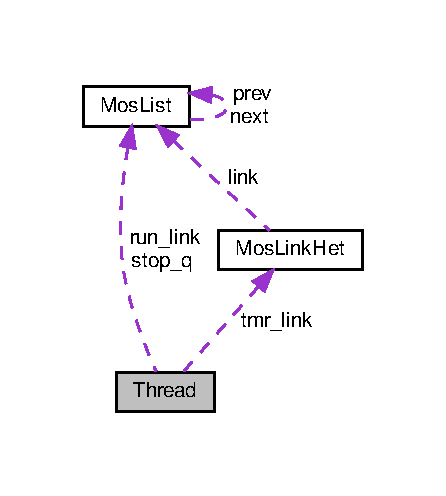
\includegraphics[width=214pt]{structThread__coll__graph}
\end{center}
\end{figure}
\subsection*{Public Attributes}
\begin{DoxyCompactItemize}
\item 
\mbox{\Hypertarget{structThread_afc3cecf6a5fd6d5017832d0457662173}\label{structThread_afc3cecf6a5fd6d5017832d0457662173}} 
u32 {\bfseries sp}
\item 
\mbox{\Hypertarget{structThread_ae691e0584e1eade245b788908f464a03}\label{structThread_ae691e0584e1eade245b788908f464a03}} 
error\+\_\+t {\bfseries err\+\_\+no}
\item 
\mbox{\Hypertarget{structThread_aac801cf519496bf4774cc0501aa8ce6b}\label{structThread_aac801cf519496bf4774cc0501aa8ce6b}} 
Thread\+State {\bfseries state}
\item 
\mbox{\Hypertarget{structThread_a37222bf9e713bee1d695549507ab5393}\label{structThread_a37222bf9e713bee1d695549507ab5393}} 
\hyperlink{structMosList}{Mos\+Link} {\bfseries run\+\_\+link}
\item 
\mbox{\Hypertarget{structThread_a9a2b54f6e60ec7d2f223864e96dcc9f5}\label{structThread_a9a2b54f6e60ec7d2f223864e96dcc9f5}} 
\hyperlink{structMosLinkHet}{Mos\+Link\+Het} {\bfseries tmr\+\_\+link}
\item 
\mbox{\Hypertarget{structThread_af3268a21afb8d448a2be3dc990504e1d}\label{structThread_af3268a21afb8d448a2be3dc990504e1d}} 
\hyperlink{structMosList}{Mos\+List} {\bfseries stop\+\_\+q}
\item 
\mbox{\Hypertarget{structThread_aea39a4e54bf67fea1a33f686b3b8a09b}\label{structThread_aea39a4e54bf67fea1a33f686b3b8a09b}} 
u32 {\bfseries wake\+\_\+tick}
\item 
\mbox{\Hypertarget{structThread_a98be222f67e6175a8757d4c085d8d8bb}\label{structThread_a98be222f67e6175a8757d4c085d8d8bb}} 
Mos\+Thread\+Priority {\bfseries pri}
\item 
\mbox{\Hypertarget{structThread_a7a4d4c35d664801210eb24c8405a0a23}\label{structThread_a7a4d4c35d664801210eb24c8405a0a23}} 
Mos\+Thread\+Priority {\bfseries nom\+\_\+pri}
\item 
\mbox{\Hypertarget{structThread_a8ed14bf5f38c37351372735d6ac659c2}\label{structThread_a8ed14bf5f38c37351372735d6ac659c2}} 
u8 {\bfseries stop\+\_\+request}
\item 
\mbox{\Hypertarget{structThread_ad45a2fe4944346e40290374fce528ef6}\label{structThread_ad45a2fe4944346e40290374fce528ef6}} 
u8 {\bfseries timed\+\_\+out}
\item 
\mbox{\Hypertarget{structThread_a87c95f46840af831c15a8d3ce4bf07f4}\label{structThread_a87c95f46840af831c15a8d3ce4bf07f4}} 
s32 {\bfseries rtn\+\_\+val}
\item 
\mbox{\Hypertarget{structThread_a3d0af2b2fdad8db046c10e424dec1f5e}\label{structThread_a3d0af2b2fdad8db046c10e424dec1f5e}} 
Mos\+Thread\+Entry $\ast$ {\bfseries term\+\_\+handler}
\item 
\mbox{\Hypertarget{structThread_ab22cfb674ca05936706e250adf61d9d9}\label{structThread_ab22cfb674ca05936706e250adf61d9d9}} 
s32 {\bfseries term\+\_\+arg}
\item 
\mbox{\Hypertarget{structThread_ad4063736b201d8cf7a550404cc215bb1}\label{structThread_ad4063736b201d8cf7a550404cc215bb1}} 
u8 $\ast$ {\bfseries stack\+\_\+bottom}
\item 
\mbox{\Hypertarget{structThread_afeaf0a58480ba57c3d63b9d50bb55141}\label{structThread_afeaf0a58480ba57c3d63b9d50bb55141}} 
u32 {\bfseries stack\+\_\+size}
\item 
\mbox{\Hypertarget{structThread_adf8367c62ce6a746d82304600cbd2f9c}\label{structThread_adf8367c62ce6a746d82304600cbd2f9c}} 
const char $\ast$ {\bfseries name}
\item 
\mbox{\Hypertarget{structThread_ae44b9fe64e38313776b5feef642a9356}\label{structThread_ae44b9fe64e38313776b5feef642a9356}} 
s32 {\bfseries ref\+\_\+cnt}
\end{DoxyCompactItemize}


The documentation for this struct was generated from the following file\+:\begin{DoxyCompactItemize}
\item 
mos/kernel.\+c\end{DoxyCompactItemize}

\hypertarget{unionTicker}{}\section{Ticker Union Reference}
\label{unionTicker}\index{Ticker@{Ticker}}
\subsection*{Public Attributes}
\begin{DoxyCompactItemize}
\item 
\mbox{\Hypertarget{unionTicker_a023a42cca05e44013b3fedccfeac32b5}\label{unionTicker_a023a42cca05e44013b3fedccfeac32b5}} 
u64 {\bfseries count}
\item 
\mbox{\Hypertarget{unionTicker_ae164d38652d655a9ed82603e0f1e7d3a}\label{unionTicker_ae164d38652d655a9ed82603e0f1e7d3a}} 
\begin{tabbing}
xx\=xx\=xx\=xx\=xx\=xx\=xx\=xx\=xx\=\kill
struct \{\\
\>u32 {\bfseries lower}\\
\>u32 {\bfseries upper}\\
\}; \\

\end{tabbing}\end{DoxyCompactItemize}


The documentation for this union was generated from the following file\+:\begin{DoxyCompactItemize}
\item 
mos/kernel.\+c\end{DoxyCompactItemize}

\chapter{File Documentation}
\hypertarget{context_8h}{}\section{mos/context.h File Reference}
\label{context_8h}\index{mos/context.\+h@{mos/context.\+h}}


Shared Contexts.  


{\ttfamily \#include $<$mos/kernel.\+h$>$}\newline
{\ttfamily \#include $<$mos/queue.\+h$>$}\newline
{\ttfamily \#include $<$mos/trace.\+h$>$}\newline
Include dependency graph for context.\+h\+:\nopagebreak
\begin{figure}[H]
\begin{center}
\leavevmode
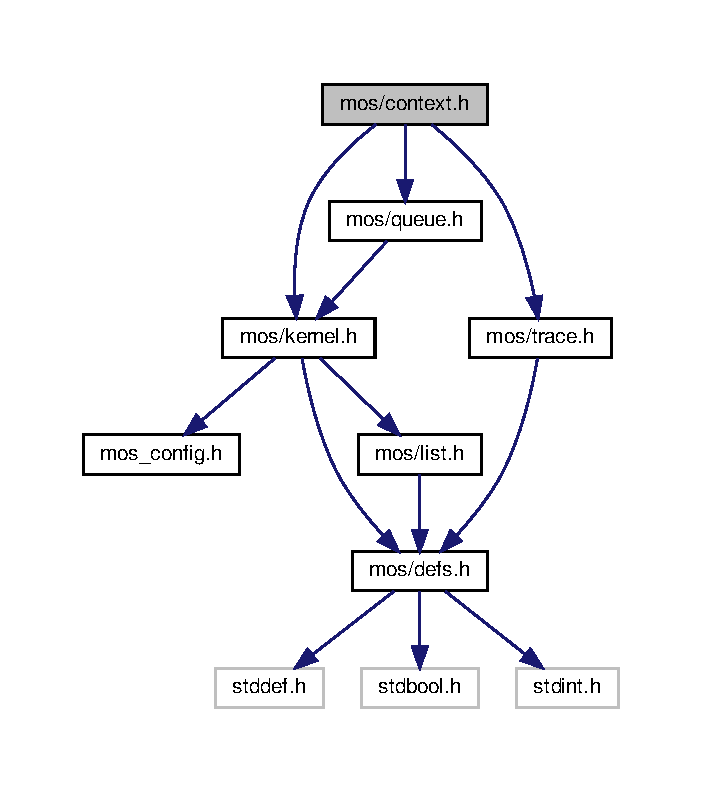
\includegraphics[width=337pt]{context_8h__incl}
\end{center}
\end{figure}
\subsection*{Classes}
\begin{DoxyCompactItemize}
\item 
struct \hyperlink{structMosContextMessage}{Mos\+Context\+Message}
\item 
struct \hyperlink{structMosClient}{Mos\+Client}
\item 
struct \hyperlink{structMosContext}{Mos\+Context}
\item 
struct \hyperlink{structMosContextTimer}{Mos\+Context\+Timer}
\end{DoxyCompactItemize}
\subsection*{Typedefs}
\begin{DoxyCompactItemize}
\item 
\mbox{\Hypertarget{context_8h_a0f5a5853b5404b549587f080762d82c0}\label{context_8h_a0f5a5853b5404b549587f080762d82c0}} 
typedef u32 {\bfseries Mos\+Context\+Message\+ID}
\item 
\mbox{\Hypertarget{context_8h_a762ad564702708ead70e0b7edf9dc8f3}\label{context_8h_a762ad564702708ead70e0b7edf9dc8f3}} 
typedef bool() {\bfseries Mos\+Client\+Handler}(\hyperlink{structMosContextMessage}{Mos\+Context\+Message} $\ast$)
\item 
\mbox{\Hypertarget{context_8h_abcf071288b0b41b19de23f4ad9be9278}\label{context_8h_abcf071288b0b41b19de23f4ad9be9278}} 
typedef struct \hyperlink{structMosClient}{Mos\+Client} {\bfseries Mos\+Client}
\end{DoxyCompactItemize}
\subsection*{Enumerations}
\begin{DoxyCompactItemize}
\item 
\mbox{\Hypertarget{context_8h_a41e6609804d83834dc1a19f92e828492}\label{context_8h_a41e6609804d83834dc1a19f92e828492}} 
enum {\bfseries Mos\+Context\+Message\+ID} \{ \newline
{\bfseries Mos\+Context\+Message\+I\+D\+\_\+\+Start\+Client} = 0x\+F\+F\+F\+F\+F\+F\+FC, 
{\bfseries Mos\+Context\+Message\+I\+D\+\_\+\+Stop\+Client} = 0x\+F\+F\+F\+F\+F\+F\+FD, 
{\bfseries Mos\+Context\+Message\+I\+D\+\_\+\+Resume\+Client} = 0x\+F\+F\+F\+F\+F\+F\+FE, 
{\bfseries Mos\+Context\+Message\+I\+D\+\_\+\+Stop\+Context} = 0x\+F\+F\+F\+F\+F\+F\+FF, 
\newline
{\bfseries Mos\+Context\+Message\+I\+D\+\_\+\+First\+User\+Message} = 0x00000000
 \}
\end{DoxyCompactItemize}
\subsection*{Functions}
\begin{DoxyCompactItemize}
\item 
\mbox{\Hypertarget{context_8h_a96873fd8971410364f0f49b20245efc2}\label{context_8h_a96873fd8971410364f0f49b20245efc2}} 
M\+O\+S\+\_\+\+C\+L\+I\+E\+N\+T\+\_\+\+U\+N\+S\+A\+FE void {\bfseries Mos\+Init\+Context} (\hyperlink{structMosContext}{Mos\+Context} $\ast$context, Mos\+Thread\+Priority prio, u8 $\ast$stack\+\_\+bottom, u32 stack\+\_\+size, \hyperlink{structMosContextMessage}{Mos\+Context\+Message} $\ast$msg\+\_\+queue\+\_\+buf, u32 msg\+\_\+queue\+\_\+depth)
\item 
\mbox{\Hypertarget{context_8h_ac6240b974e98bbdd2b3d56b0e5625442}\label{context_8h_ac6240b974e98bbdd2b3d56b0e5625442}} 
M\+O\+S\+\_\+\+C\+L\+I\+E\+N\+T\+\_\+\+U\+N\+S\+A\+FE void {\bfseries Mos\+Start\+Context} (\hyperlink{structMosContext}{Mos\+Context} $\ast$context)
\item 
\mbox{\Hypertarget{context_8h_ac11f2b251810f7991bf5b2b92ec4a57f}\label{context_8h_ac11f2b251810f7991bf5b2b92ec4a57f}} 
M\+O\+S\+\_\+\+C\+L\+I\+E\+N\+T\+\_\+\+U\+N\+S\+A\+FE void {\bfseries Mos\+Stop\+Context} (\hyperlink{structMosContext}{Mos\+Context} $\ast$context)
\item 
\mbox{\Hypertarget{context_8h_aa46e2b7a2cbb13db129414450ba70b00}\label{context_8h_aa46e2b7a2cbb13db129414450ba70b00}} 
M\+O\+S\+\_\+\+C\+L\+I\+E\+N\+T\+\_\+\+U\+N\+S\+A\+FE void {\bfseries Mos\+Wait\+For\+Context\+Stop} (\hyperlink{structMosContext}{Mos\+Context} $\ast$context)
\item 
\mbox{\Hypertarget{context_8h_af3e9ac5ba76d2926ed6216e1389bb2b6}\label{context_8h_af3e9ac5ba76d2926ed6216e1389bb2b6}} 
M\+O\+S\+\_\+\+C\+L\+I\+E\+N\+T\+\_\+\+U\+N\+S\+A\+FE void {\bfseries Mos\+Start\+Client} (\hyperlink{structMosContext}{Mos\+Context} $\ast$context, \hyperlink{structMosClient}{Mos\+Client} $\ast$client, Mos\+Client\+Handler $\ast$handler, void $\ast$priv\+\_\+data)
\item 
\mbox{\Hypertarget{context_8h_a86b994bbd386c225198fb7a28640f56e}\label{context_8h_a86b994bbd386c225198fb7a28640f56e}} 
M\+O\+S\+\_\+\+C\+L\+I\+E\+N\+T\+\_\+\+U\+N\+S\+A\+FE void {\bfseries Mos\+Stop\+Client} (\hyperlink{structMosContext}{Mos\+Context} $\ast$context, \hyperlink{structMosClient}{Mos\+Client} $\ast$client)
\item 
\mbox{\Hypertarget{context_8h_a6bd8d3e555c9f18cca96dda0419b3f46}\label{context_8h_a6bd8d3e555c9f18cca96dda0419b3f46}} 
M\+O\+S\+\_\+\+I\+S\+R\+\_\+\+S\+A\+FE M\+O\+S\+\_\+\+I\+N\+L\+I\+NE void {\bfseries Mos\+Set\+Context\+Message} (\hyperlink{structMosContextMessage}{Mos\+Context\+Message} $\ast$msg, \hyperlink{structMosClient}{Mos\+Client} $\ast$client, Mos\+Context\+Message\+ID id)
\item 
\mbox{\Hypertarget{context_8h_a6e60f6d8855e6ec1a543bc85f408afa3}\label{context_8h_a6e60f6d8855e6ec1a543bc85f408afa3}} 
M\+O\+S\+\_\+\+I\+S\+R\+\_\+\+S\+A\+FE M\+O\+S\+\_\+\+I\+N\+L\+I\+NE void {\bfseries Mos\+Set\+Context\+Broadcast\+Message} (\hyperlink{structMosContextMessage}{Mos\+Context\+Message} $\ast$msg, Mos\+Context\+Message\+ID id)
\item 
\mbox{\Hypertarget{context_8h_aeadf0881d123527759698865866a2b69}\label{context_8h_aeadf0881d123527759698865866a2b69}} 
M\+O\+S\+\_\+\+I\+S\+R\+\_\+\+S\+A\+FE M\+O\+S\+\_\+\+I\+N\+L\+I\+NE void {\bfseries Mos\+Set\+Context\+Message\+Data} (\hyperlink{structMosContextMessage}{Mos\+Context\+Message} $\ast$msg, void $\ast$data)
\item 
\mbox{\Hypertarget{context_8h_a8d50a51799615d42668d58ee132c91ff}\label{context_8h_a8d50a51799615d42668d58ee132c91ff}} 
M\+O\+S\+\_\+\+I\+S\+R\+\_\+\+S\+A\+FE M\+O\+S\+\_\+\+I\+N\+L\+I\+NE bool {\bfseries Mos\+Try\+Send\+Message\+To\+Context} (\hyperlink{structMosContext}{Mos\+Context} $\ast$context, \hyperlink{structMosContextMessage}{Mos\+Context\+Message} $\ast$msg)
\item 
\mbox{\Hypertarget{context_8h_abb8bbb14dfac4db77c431c91f8b6a4d2}\label{context_8h_abb8bbb14dfac4db77c431c91f8b6a4d2}} 
M\+O\+S\+\_\+\+I\+N\+L\+I\+NE void {\bfseries Mos\+Send\+Message\+To\+Context} (\hyperlink{structMosContext}{Mos\+Context} $\ast$context, \hyperlink{structMosContextMessage}{Mos\+Context\+Message} $\ast$msg)
\item 
\mbox{\Hypertarget{context_8h_a1a25826ddaac2d265bd7c8ed47e13981}\label{context_8h_a1a25826ddaac2d265bd7c8ed47e13981}} 
void {\bfseries Mos\+Init\+Context\+Timer} (\hyperlink{structMosContextTimer}{Mos\+Context\+Timer} $\ast$tmr, \hyperlink{structMosContext}{Mos\+Context} $\ast$context)
\item 
\mbox{\Hypertarget{context_8h_a5431ec458899ef7c0a89fa6f6561f74f}\label{context_8h_a5431ec458899ef7c0a89fa6f6561f74f}} 
M\+O\+S\+\_\+\+I\+N\+L\+I\+NE void {\bfseries Mos\+Set\+Context\+Timer} (\hyperlink{structMosContextTimer}{Mos\+Context\+Timer} $\ast$tmr, u32 ticks, \hyperlink{structMosContextMessage}{Mos\+Context\+Message} $\ast$msg)
\item 
\mbox{\Hypertarget{context_8h_a8ae38a2929592a2651c63988c54c86b7}\label{context_8h_a8ae38a2929592a2651c63988c54c86b7}} 
M\+O\+S\+\_\+\+I\+N\+L\+I\+NE void {\bfseries Mos\+Cancel\+Context\+Timer} (\hyperlink{structMosContextTimer}{Mos\+Context\+Timer} $\ast$tmr)
\item 
\mbox{\Hypertarget{context_8h_a65d86ac9d993f0adb3c8a93d00dc2228}\label{context_8h_a65d86ac9d993f0adb3c8a93d00dc2228}} 
M\+O\+S\+\_\+\+I\+N\+L\+I\+NE void {\bfseries Mos\+Reset\+Context\+Timer} (\hyperlink{structMosContextTimer}{Mos\+Context\+Timer} $\ast$tmr)
\end{DoxyCompactItemize}


\subsection{Detailed Description}
Shared Contexts. 

Shared contexts allow multiple client modules to share the same resources, including a single run thread, thread stack and message queue. In addition, shared contexts can reduce or eliminate mutex contention since clients in the same shared context are guaranteed to not preempt each other. In general, shared contexts should be implemented at lower thread priorities than most other functionality. Think of contexts as a form of cooperative multitasking where memory savings are a lot more important than deadlines.

Contexts use a shared message queue for inter-\/client communication. The maximum latency depends on the maximum processing time for all messages in the context. Context clients should be implemented as state machines that multiplex received messages. Contexts can send and receive messages to or from I\+S\+Rs or other threads on the system. Clients should not block or wait very long otherwise they might starve other clients sharing the same context. The Mos\+Try\+Send\+Message\+To\+Context() call should be used when a client sends a message to another client in the same context.

If a client handler has not completed and desires a callback, it should return false. Note that the callback is implemented as a resume message on the same message queue. The resume message will be added to the end of the queue allowing the opportunity for other messages to drain first.

Client handlers state machines should tolerate receiving messages after being {\itshape individually} stopped. This includes, but is not limited to broadcast stop messages, resume messages or potentially even user messages (depending on the system design and how the context is used).

The overall context will only shutdown upon receipt of a {\itshape broadcast} Stop\+Context message and any messages that are queued beyond a {\itshape broadcast} Stop\+Contextmessage will be ignored. Any clients requesting resume after receiving a broadcast Stop\+Context stop message will also be ignored. All clients will receive a Stop\+Client message upon receipt of a {\itshape broadcast} Stop\+Context message (even if already stopped). 
\hypertarget{heap_8h}{}\section{mos/heap.h File Reference}
\label{heap_8h}\index{mos/heap.\+h@{mos/heap.\+h}}


M\+OS Heap.  


{\ttfamily \#include $<$mos/kernel.\+h$>$}\newline
Include dependency graph for heap.\+h\+:\nopagebreak
\begin{figure}[H]
\begin{center}
\leavevmode
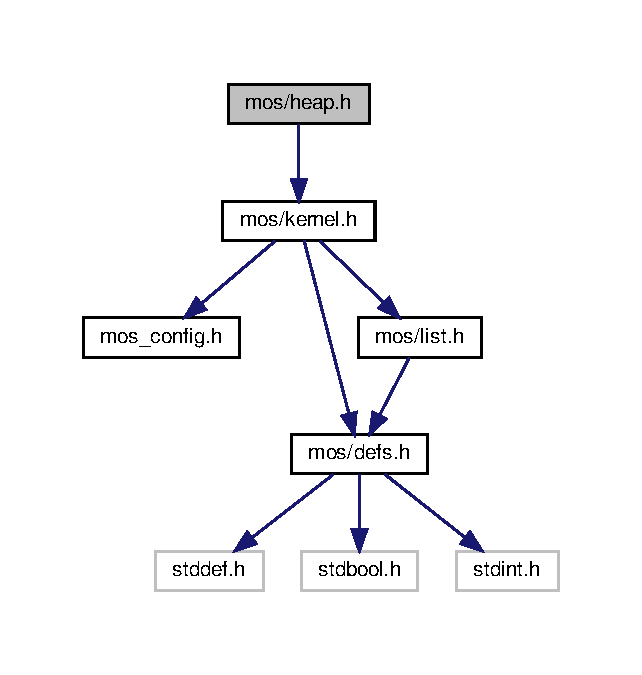
\includegraphics[width=308pt]{heap_8h__incl}
\end{center}
\end{figure}
This graph shows which files directly or indirectly include this file\+:\nopagebreak
\begin{figure}[H]
\begin{center}
\leavevmode
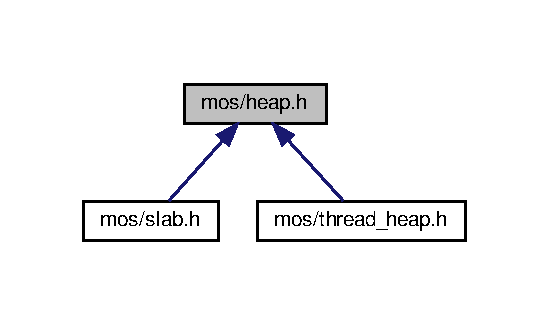
\includegraphics[width=264pt]{heap_8h__dep__incl}
\end{center}
\end{figure}
\subsection*{Classes}
\begin{DoxyCompactItemize}
\item 
struct \hyperlink{structMosHeap}{Mos\+Heap}
\end{DoxyCompactItemize}
\subsection*{Functions}
\begin{DoxyCompactItemize}
\item 
\mbox{\Hypertarget{heap_8h_ab0138811c0d8ead01fa285ef967bc50c}\label{heap_8h_ab0138811c0d8ead01fa285ef967bc50c}} 
void {\bfseries Mos\+Init\+Heap} (\hyperlink{structMosHeap}{Mos\+Heap} $\ast$heap, u8 $\ast$data, u32 heap\+\_\+size, u32 alignment)
\item 
\mbox{\Hypertarget{heap_8h_a16f31a3bedd7620adb6b2cd16fb4c3db}\label{heap_8h_a16f31a3bedd7620adb6b2cd16fb4c3db}} 
void $\ast$ {\bfseries Mos\+Alloc} (\hyperlink{structMosHeap}{Mos\+Heap} $\ast$heap, u32 size)
\item 
\mbox{\Hypertarget{heap_8h_a11d84d50bbcfd29cf2dfd622a63c0d38}\label{heap_8h_a11d84d50bbcfd29cf2dfd622a63c0d38}} 
void $\ast$ {\bfseries Mos\+Re\+Alloc} (\hyperlink{structMosHeap}{Mos\+Heap} $\ast$heap, void $\ast$block, u32 new\+\_\+size)
\item 
\mbox{\Hypertarget{heap_8h_a34506fd706b3499b7a9d82307f834276}\label{heap_8h_a34506fd706b3499b7a9d82307f834276}} 
void {\bfseries Mos\+Free} (\hyperlink{structMosHeap}{Mos\+Heap} $\ast$heap, void $\ast$block)
\end{DoxyCompactItemize}


\subsection{Detailed Description}
M\+OS Heap. 


\hypertarget{kernel_8h}{}\section{mos/kernel.h File Reference}
\label{kernel_8h}\index{mos/kernel.\+h@{mos/kernel.\+h}}


M\+OS Microkernel.  


{\ttfamily \#include \char`\"{}mos\+\_\+config.\+h\char`\"{}}\newline
{\ttfamily \#include $<$mos/defs.\+h$>$}\newline
{\ttfamily \#include $<$mos/list.\+h$>$}\newline
Include dependency graph for kernel.\+h\+:\nopagebreak
\begin{figure}[H]
\begin{center}
\leavevmode
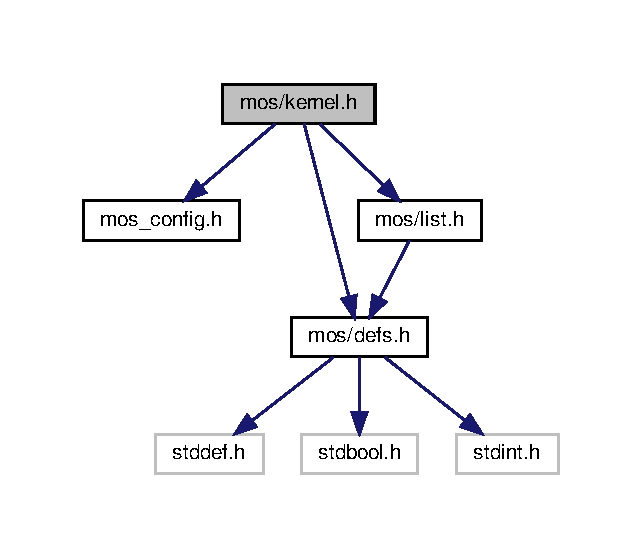
\includegraphics[width=308pt]{kernel_8h__incl}
\end{center}
\end{figure}
This graph shows which files directly or indirectly include this file\+:\nopagebreak
\begin{figure}[H]
\begin{center}
\leavevmode
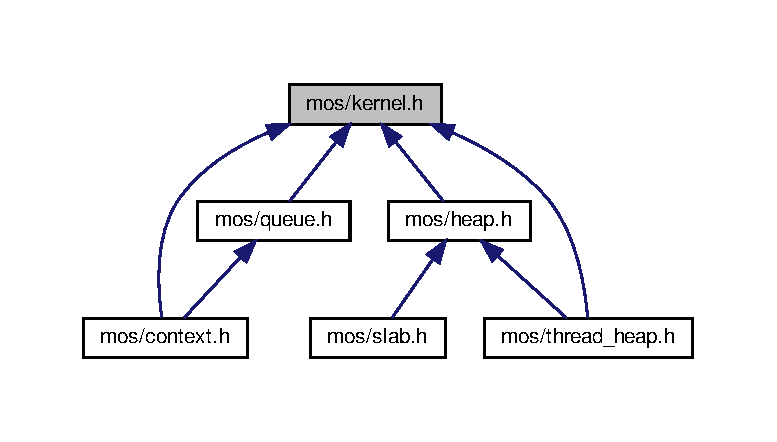
\includegraphics[width=350pt]{kernel_8h__dep__incl}
\end{center}
\end{figure}
\subsection*{Classes}
\begin{DoxyCompactItemize}
\item 
struct \hyperlink{structMosParams}{Mos\+Params}
\item 
struct \hyperlink{structMosThread}{Mos\+Thread}
\item 
struct \hyperlink{structMosMutex}{Mos\+Mutex}
\item 
struct \hyperlink{structMosSem}{Mos\+Sem}
\item 
struct \hyperlink{structMosTimer}{Mos\+Timer}
\end{DoxyCompactItemize}
\subsection*{Macros}
\begin{DoxyCompactItemize}
\item 
\mbox{\Hypertarget{kernel_8h_a5f29167fe17925a61f0509a83d951f2b}\label{kernel_8h_a5f29167fe17925a61f0509a83d951f2b}} 
\#define {\bfseries Mos\+Assert}(c)
\end{DoxyCompactItemize}
\subsection*{Typedefs}
\begin{DoxyCompactItemize}
\item 
\mbox{\Hypertarget{kernel_8h_aa5050bca48e0baf57e0594e7926b7dff}\label{kernel_8h_aa5050bca48e0baf57e0594e7926b7dff}} 
typedef struct \hyperlink{structMosTimer}{Mos\+Timer} {\bfseries Mos\+Timer}
\item 
\mbox{\Hypertarget{kernel_8h_a95cd5faf8ba49c469711ee8fee68ca14}\label{kernel_8h_a95cd5faf8ba49c469711ee8fee68ca14}} 
typedef s32() {\bfseries Mos\+Thread\+Entry}(s32 arg)
\item 
\mbox{\Hypertarget{kernel_8h_a8ce2b68073e027dc190217ea8039bc80}\label{kernel_8h_a8ce2b68073e027dc190217ea8039bc80}} 
typedef M\+O\+S\+\_\+\+I\+S\+R\+\_\+\+S\+A\+FE bool() {\bfseries Mos\+Timer\+Callback}(\hyperlink{structMosTimer}{Mos\+Timer} $\ast$tmr)
\item 
\mbox{\Hypertarget{kernel_8h_a1c54c1f2e2f0b84d3150e135565f95c8}\label{kernel_8h_a1c54c1f2e2f0b84d3150e135565f95c8}} 
typedef void() {\bfseries Mos\+Raw\+Printf\+Hook}(const char $\ast$fmt,...)
\item 
\mbox{\Hypertarget{kernel_8h_aeb7c1de03bb34b7dfdf856d990be1839}\label{kernel_8h_aeb7c1de03bb34b7dfdf856d990be1839}} 
typedef void() {\bfseries Mos\+Sleep\+Hook}(void)
\item 
\mbox{\Hypertarget{kernel_8h_a9939de904ab45cd1e50d513757212d13}\label{kernel_8h_a9939de904ab45cd1e50d513757212d13}} 
typedef void() {\bfseries Mos\+Wake\+Hook}(void)
\item 
\mbox{\Hypertarget{kernel_8h_ab387c0d2e06b391ce834719cd23749d7}\label{kernel_8h_ab387c0d2e06b391ce834719cd23749d7}} 
typedef void() {\bfseries Mos\+Event\+Hook}(Mos\+Event evt, u32 val)
\item 
\mbox{\Hypertarget{kernel_8h_a1cc3d474070714b392714656ee2aac18}\label{kernel_8h_a1cc3d474070714b392714656ee2aac18}} 
typedef struct \hyperlink{structMosParams}{Mos\+Params} {\bfseries Mos\+Params}
\item 
\mbox{\Hypertarget{kernel_8h_a14e38e521609eaa89557e25a79048a2a}\label{kernel_8h_a14e38e521609eaa89557e25a79048a2a}} 
typedef struct \hyperlink{structMosThread}{Mos\+Thread} {\bfseries Mos\+Thread}
\item 
\mbox{\Hypertarget{kernel_8h_a1d40c8e34008598fb61afa478a60cfd8}\label{kernel_8h_a1d40c8e34008598fb61afa478a60cfd8}} 
typedef struct \hyperlink{structMosMutex}{Mos\+Mutex} {\bfseries Mos\+Mutex}
\item 
\mbox{\Hypertarget{kernel_8h_a6d1ceed14893767141afef7e83c38c66}\label{kernel_8h_a6d1ceed14893767141afef7e83c38c66}} 
typedef struct \hyperlink{structMosSem}{Mos\+Sem} {\bfseries Mos\+Sem}
\item 
\mbox{\Hypertarget{kernel_8h_a2bd6b2c0ed5c03a5e2f8d621f64ac182}\label{kernel_8h_a2bd6b2c0ed5c03a5e2f8d621f64ac182}} 
typedef \hyperlink{structMosSem}{Mos\+Sem} {\bfseries Mos\+Signal}
\end{DoxyCompactItemize}
\subsection*{Enumerations}
\begin{DoxyCompactItemize}
\item 
\mbox{\Hypertarget{kernel_8h_a487d0828b9aea025af245f92e69e878b}\label{kernel_8h_a487d0828b9aea025af245f92e69e878b}} 
enum {\bfseries Mos\+Thread\+State} \{ {\bfseries M\+O\+S\+\_\+\+T\+H\+R\+E\+A\+D\+\_\+\+N\+O\+T\+\_\+\+S\+T\+A\+R\+T\+ED}, 
{\bfseries M\+O\+S\+\_\+\+T\+H\+R\+E\+A\+D\+\_\+\+R\+U\+N\+N\+I\+NG}, 
{\bfseries M\+O\+S\+\_\+\+T\+H\+R\+E\+A\+D\+\_\+\+S\+T\+O\+P\+\_\+\+R\+E\+Q\+U\+E\+ST}, 
{\bfseries M\+O\+S\+\_\+\+T\+H\+R\+E\+A\+D\+\_\+\+S\+T\+O\+P\+P\+ED}
 \}
\item 
\mbox{\Hypertarget{kernel_8h_a3dc6756da9698407608ffa75ba0dd94a}\label{kernel_8h_a3dc6756da9698407608ffa75ba0dd94a}} 
enum {\bfseries Mos\+Event} \{ {\bfseries M\+O\+S\+\_\+\+E\+V\+E\+N\+T\+\_\+\+S\+C\+H\+E\+D\+U\+L\+E\+R\+\_\+\+E\+N\+T\+RY}, 
{\bfseries M\+O\+S\+\_\+\+E\+V\+E\+N\+T\+\_\+\+S\+C\+H\+E\+D\+U\+L\+E\+R\+\_\+\+E\+X\+IT}, 
{\bfseries M\+O\+S\+\_\+\+E\+V\+E\+N\+T\+\_\+\+T\+I\+CK}
 \}
\end{DoxyCompactItemize}
\subsection*{Functions}
\begin{DoxyCompactItemize}
\item 
void \hyperlink{kernel_8h_ac627e1bcc2148407e4b9651edacbe9f5}{Mos\+Init} (void)
\item 
void \hyperlink{kernel_8h_a00f08c404afd055260ca28420d924cf9}{Mos\+Run\+Scheduler} (void)
\item 
\mbox{\Hypertarget{kernel_8h_a731b146234a671bee7572dd465ea7c77}\label{kernel_8h_a731b146234a671bee7572dd465ea7c77}} 
void {\bfseries Mos\+Register\+Raw\+Printf\+Hook} (Mos\+Raw\+Printf\+Hook $\ast$hook)
\item 
\mbox{\Hypertarget{kernel_8h_a6189c22469de79028ff307bcc1b66c47}\label{kernel_8h_a6189c22469de79028ff307bcc1b66c47}} 
void {\bfseries Mos\+Register\+Sleep\+Hook} (Mos\+Sleep\+Hook $\ast$hook)
\item 
\mbox{\Hypertarget{kernel_8h_a09dabc06b4b90e3cd1e2393cb82927dd}\label{kernel_8h_a09dabc06b4b90e3cd1e2393cb82927dd}} 
void {\bfseries Mos\+Register\+Wake\+Hook} (Mos\+Wake\+Hook $\ast$hook)
\item 
\mbox{\Hypertarget{kernel_8h_a42652241f6db615ebf88185a2f9bc5c4}\label{kernel_8h_a42652241f6db615ebf88185a2f9bc5c4}} 
void {\bfseries Mos\+Register\+Event\+Hook} (Mos\+Event\+Hook $\ast$hook)
\item 
const \hyperlink{structMosParams}{Mos\+Params} $\ast$ \hyperlink{kernel_8h_adc534b28b36d8cade3943f95a6c9d10c}{Mos\+Get\+Params} (void)
\item 
static M\+O\+S\+\_\+\+I\+N\+L\+I\+NE u32 M\+O\+S\+\_\+\+I\+S\+R\+\_\+\+S\+A\+FE \hyperlink{kernel_8h_ab69b30c32bde430d808fe0973e3718b2}{Mos\+Get\+I\+R\+Q\+Number} (void)
\item 
\mbox{\Hypertarget{kernel_8h_acf034091c69f31846062d7cf758b6392}\label{kernel_8h_acf034091c69f31846062d7cf758b6392}} 
M\+O\+S\+\_\+\+I\+S\+R\+\_\+\+S\+A\+FE void {\bfseries Mos\+Disable\+Interrupts} (void)
\item 
\mbox{\Hypertarget{kernel_8h_a6ef4fe0b6dbf0319de975c720631bfcc}\label{kernel_8h_a6ef4fe0b6dbf0319de975c720631bfcc}} 
M\+O\+S\+\_\+\+I\+S\+R\+\_\+\+S\+A\+FE void {\bfseries Mos\+Enable\+Interrupts} (void)
\item 
\mbox{\Hypertarget{kernel_8h_a7b5f4e5407c3651b246d1e3fc9955633}\label{kernel_8h_a7b5f4e5407c3651b246d1e3fc9955633}} 
M\+O\+S\+\_\+\+I\+S\+R\+\_\+\+S\+A\+FE u32 {\bfseries Mos\+Get\+Tick\+Count} (void)
\item 
\mbox{\Hypertarget{kernel_8h_aaab41ad34da7d34d2c1aea893594a316}\label{kernel_8h_aaab41ad34da7d34d2c1aea893594a316}} 
M\+O\+S\+\_\+\+I\+S\+R\+\_\+\+S\+A\+FE u64 {\bfseries Mos\+Get\+Cycle\+Count} (void)
\item 
\mbox{\Hypertarget{kernel_8h_a793b2ddb0ab1c4cd01038b33c67002c3}\label{kernel_8h_a793b2ddb0ab1c4cd01038b33c67002c3}} 
void {\bfseries Mos\+Advance\+Tick\+Count} (u32 ticks)
\item 
\mbox{\Hypertarget{kernel_8h_aa13a3569908f14115aaf28136a744dab}\label{kernel_8h_aa13a3569908f14115aaf28136a744dab}} 
void {\bfseries Mos\+Delay\+Thread} (u32 ticks)
\item 
\mbox{\Hypertarget{kernel_8h_ae7f01ab27571ca6807600f4f8b823157}\label{kernel_8h_ae7f01ab27571ca6807600f4f8b823157}} 
M\+O\+S\+\_\+\+I\+S\+R\+\_\+\+S\+A\+FE void {\bfseries Mos\+Delay\+Micro\+Sec} (u32 usec)
\item 
\mbox{\Hypertarget{kernel_8h_ad8c28fe8618c75e75c562d232a3d984a}\label{kernel_8h_ad8c28fe8618c75e75c562d232a3d984a}} 
void {\bfseries Mos\+Init\+Timer} (\hyperlink{structMosTimer}{Mos\+Timer} $\ast$tmr, Mos\+Timer\+Callback $\ast$callback)
\item 
\mbox{\Hypertarget{kernel_8h_af0984a544afb42ee114dd5e977d0f7a9}\label{kernel_8h_af0984a544afb42ee114dd5e977d0f7a9}} 
void {\bfseries Mos\+Set\+Timer} (\hyperlink{structMosTimer}{Mos\+Timer} $\ast$tmr, u32 ticks, void $\ast$priv\+\_\+data)
\item 
\mbox{\Hypertarget{kernel_8h_afdb07077e4e033263a7187519ac14f4b}\label{kernel_8h_afdb07077e4e033263a7187519ac14f4b}} 
void {\bfseries Mos\+Cancel\+Timer} (\hyperlink{structMosTimer}{Mos\+Timer} $\ast$tmr)
\item 
\mbox{\Hypertarget{kernel_8h_a925608235c413d8bd37dee757c4dbc7d}\label{kernel_8h_a925608235c413d8bd37dee757c4dbc7d}} 
void {\bfseries Mos\+Reset\+Timer} (\hyperlink{structMosTimer}{Mos\+Timer} $\ast$tmr)
\item 
\mbox{\Hypertarget{kernel_8h_a2d656e70d3518ecf23a0c5f2e8195181}\label{kernel_8h_a2d656e70d3518ecf23a0c5f2e8195181}} 
M\+O\+S\+\_\+\+I\+S\+R\+\_\+\+S\+A\+FE void {\bfseries Mos\+Yield\+Thread} (void)
\item 
\mbox{\Hypertarget{kernel_8h_ace9403da615861e7f804387d09c320bd}\label{kernel_8h_ace9403da615861e7f804387d09c320bd}} 
\hyperlink{structMosThread}{Mos\+Thread} $\ast$ {\bfseries Mos\+Get\+Thread\+Ptr} (void)
\item 
\mbox{\Hypertarget{kernel_8h_a7abef23b2789a391f43ba9c3b55d73a6}\label{kernel_8h_a7abef23b2789a391f43ba9c3b55d73a6}} 
static M\+O\+S\+\_\+\+I\+N\+L\+I\+NE u32 {\bfseries Mos\+Get\+Stack\+Depth} (u8 $\ast$top)
\item 
\mbox{\Hypertarget{kernel_8h_a8334e1a4a864fee38f91a5bfdf234bb1}\label{kernel_8h_a8334e1a4a864fee38f91a5bfdf234bb1}} 
void {\bfseries Mos\+Get\+Stack\+Stats} (\hyperlink{structMosThread}{Mos\+Thread} $\ast$thd, u32 $\ast$stack\+\_\+size, u32 $\ast$stack\+\_\+usage, u32 $\ast$max\+\_\+stack\+\_\+usage)
\item 
\mbox{\Hypertarget{kernel_8h_afc11f2c46072ce07830d25ba95fe6504}\label{kernel_8h_afc11f2c46072ce07830d25ba95fe6504}} 
u8 $\ast$ {\bfseries Mos\+Get\+Stack\+Bottom} (\hyperlink{structMosThread}{Mos\+Thread} $\ast$thd)
\item 
\mbox{\Hypertarget{kernel_8h_af1e7128efc90c6dffd37b40ca2cdf504}\label{kernel_8h_af1e7128efc90c6dffd37b40ca2cdf504}} 
u32 {\bfseries Mos\+Get\+Stack\+Size} (\hyperlink{structMosThread}{Mos\+Thread} $\ast$thd)
\item 
\mbox{\Hypertarget{kernel_8h_ac38420f870bdcda3be5afe518e4ee8de}\label{kernel_8h_ac38420f870bdcda3be5afe518e4ee8de}} 
void {\bfseries Mos\+Set\+Stack} (\hyperlink{structMosThread}{Mos\+Thread} $\ast$thd, u8 $\ast$stack\+\_\+bottom, u32 stack\+\_\+size)
\item 
\mbox{\Hypertarget{kernel_8h_aabbea4cb48ccffc7271839206c239d75}\label{kernel_8h_aabbea4cb48ccffc7271839206c239d75}} 
void {\bfseries Mos\+Set\+Thread\+Name} (\hyperlink{structMosThread}{Mos\+Thread} $\ast$thd, const char $\ast$name)
\item 
\mbox{\Hypertarget{kernel_8h_affb81d702b95aa062ed0fff4adfa397f}\label{kernel_8h_affb81d702b95aa062ed0fff4adfa397f}} 
bool {\bfseries Mos\+Init\+Thread} (\hyperlink{structMosThread}{Mos\+Thread} $\ast$thd, Mos\+Thread\+Priority pri, Mos\+Thread\+Entry $\ast$entry, s32 arg, u8 $\ast$stack\+\_\+bottom, u32 stack\+\_\+size)
\item 
\mbox{\Hypertarget{kernel_8h_a76e46295a3c77b18771d324bc4a7eaae}\label{kernel_8h_a76e46295a3c77b18771d324bc4a7eaae}} 
bool {\bfseries Mos\+Run\+Thread} (\hyperlink{structMosThread}{Mos\+Thread} $\ast$thd)
\item 
\mbox{\Hypertarget{kernel_8h_acc38405f58c24ef81600ab737f5f926a}\label{kernel_8h_acc38405f58c24ef81600ab737f5f926a}} 
bool {\bfseries Mos\+Init\+And\+Run\+Thread} (\hyperlink{structMosThread}{Mos\+Thread} $\ast$thd, Mos\+Thread\+Priority pri, Mos\+Thread\+Entry $\ast$entry, s32 arg, u8 $\ast$stack\+\_\+bottom, u32 stack\+\_\+size)
\item 
\mbox{\Hypertarget{kernel_8h_a74822d90b96452990884a108e0140dba}\label{kernel_8h_a74822d90b96452990884a108e0140dba}} 
Mos\+Thread\+State {\bfseries Mos\+Get\+Thread\+State} (\hyperlink{structMosThread}{Mos\+Thread} $\ast$thd, s32 $\ast$rtn\+\_\+val)
\item 
\mbox{\Hypertarget{kernel_8h_aba913d1abd4a5cf2caaf46f914318656}\label{kernel_8h_aba913d1abd4a5cf2caaf46f914318656}} 
Mos\+Thread\+Priority {\bfseries Mos\+Get\+Thread\+Priority} (\hyperlink{structMosThread}{Mos\+Thread} $\ast$thd)
\item 
\mbox{\Hypertarget{kernel_8h_aa2ceceec25ec30fd21885af7557dc152}\label{kernel_8h_aa2ceceec25ec30fd21885af7557dc152}} 
void {\bfseries Mos\+Change\+Thread\+Priority} (\hyperlink{structMosThread}{Mos\+Thread} $\ast$thd, Mos\+Thread\+Priority pri)
\item 
\mbox{\Hypertarget{kernel_8h_a505b0cfaf6374fd3e947f854b2dadd41}\label{kernel_8h_a505b0cfaf6374fd3e947f854b2dadd41}} 
void {\bfseries Mos\+Request\+Thread\+Stop} (\hyperlink{structMosThread}{Mos\+Thread} $\ast$thd)
\item 
\mbox{\Hypertarget{kernel_8h_ab8556cc31d3323e863d4735d83e63a71}\label{kernel_8h_ab8556cc31d3323e863d4735d83e63a71}} 
bool {\bfseries Mos\+Is\+Stop\+Requested} (void)
\item 
\mbox{\Hypertarget{kernel_8h_a8289c29ae3ce8c6063d59af8cfd9e5f5}\label{kernel_8h_a8289c29ae3ce8c6063d59af8cfd9e5f5}} 
s32 {\bfseries Mos\+Wait\+For\+Thread\+Stop} (\hyperlink{structMosThread}{Mos\+Thread} $\ast$thd)
\item 
\mbox{\Hypertarget{kernel_8h_a85ffc617755be492cb2f087ebaccf9db}\label{kernel_8h_a85ffc617755be492cb2f087ebaccf9db}} 
bool {\bfseries Mos\+Wait\+For\+Thread\+Stop\+Or\+TO} (\hyperlink{structMosThread}{Mos\+Thread} $\ast$thd, s32 $\ast$rtn\+\_\+val, u32 ticks)
\item 
\mbox{\Hypertarget{kernel_8h_a993497c87d6c152a83c49f6b805cba05}\label{kernel_8h_a993497c87d6c152a83c49f6b805cba05}} 
void {\bfseries Mos\+Kill\+Thread} (\hyperlink{structMosThread}{Mos\+Thread} $\ast$thd)
\item 
\mbox{\Hypertarget{kernel_8h_aed82fafb29aff6c8e8105bd9f93f82de}\label{kernel_8h_aed82fafb29aff6c8e8105bd9f93f82de}} 
void {\bfseries Mos\+Set\+Term\+Handler} (\hyperlink{structMosThread}{Mos\+Thread} $\ast$thd, Mos\+Thread\+Entry $\ast$entry, s32 arg)
\item 
\mbox{\Hypertarget{kernel_8h_a12c2e2b78a250a4501755b6e2787767a}\label{kernel_8h_a12c2e2b78a250a4501755b6e2787767a}} 
void {\bfseries Mos\+Set\+Term\+Arg} (\hyperlink{structMosThread}{Mos\+Thread} $\ast$thd, s32 arg)
\item 
\mbox{\Hypertarget{kernel_8h_a1942e2b9c55fe7d71a6805eee58491db}\label{kernel_8h_a1942e2b9c55fe7d71a6805eee58491db}} 
void {\bfseries Mos\+Init\+Mutex} (\hyperlink{structMosMutex}{Mos\+Mutex} $\ast$mtx)
\item 
\mbox{\Hypertarget{kernel_8h_aac22e1184c00a21f3ac74c877986572e}\label{kernel_8h_aac22e1184c00a21f3ac74c877986572e}} 
void {\bfseries Mos\+Lock\+Mutex} (\hyperlink{structMosMutex}{Mos\+Mutex} $\ast$mtx)
\item 
\mbox{\Hypertarget{kernel_8h_af1b840d6be1fbb7a485b3dce28cf93e5}\label{kernel_8h_af1b840d6be1fbb7a485b3dce28cf93e5}} 
bool {\bfseries Mos\+Try\+Mutex} (\hyperlink{structMosMutex}{Mos\+Mutex} $\ast$mtx)
\item 
\mbox{\Hypertarget{kernel_8h_ace1ead7810ea83c18943c153be6fa830}\label{kernel_8h_ace1ead7810ea83c18943c153be6fa830}} 
void {\bfseries Mos\+Unlock\+Mutex} (\hyperlink{structMosMutex}{Mos\+Mutex} $\ast$mtx)
\item 
\mbox{\Hypertarget{kernel_8h_a5d7111922d92d65825b5d75e516ff50c}\label{kernel_8h_a5d7111922d92d65825b5d75e516ff50c}} 
void {\bfseries Mos\+Restore\+Mutex} (\hyperlink{structMosMutex}{Mos\+Mutex} $\ast$mtx)
\item 
\mbox{\Hypertarget{kernel_8h_a267fcf53a5d9ae33b7480535a886a313}\label{kernel_8h_a267fcf53a5d9ae33b7480535a886a313}} 
bool {\bfseries Mos\+Is\+Mutex\+Owner} (\hyperlink{structMosMutex}{Mos\+Mutex} $\ast$mtx)
\item 
\mbox{\Hypertarget{kernel_8h_ab5bbc18fd3812001a949bfabe3af4199}\label{kernel_8h_ab5bbc18fd3812001a949bfabe3af4199}} 
void {\bfseries Mos\+Init\+Sem} (\hyperlink{structMosSem}{Mos\+Sem} $\ast$sem, u32 start\+\_\+value)
\item 
\mbox{\Hypertarget{kernel_8h_a0fc8c63aa86d205d6e02cbd0054694b5}\label{kernel_8h_a0fc8c63aa86d205d6e02cbd0054694b5}} 
void {\bfseries Mos\+Wait\+For\+Sem} (\hyperlink{structMosSem}{Mos\+Sem} $\ast$sem)
\item 
\mbox{\Hypertarget{kernel_8h_acbed5add0417eea2881479f2731ebfce}\label{kernel_8h_acbed5add0417eea2881479f2731ebfce}} 
bool {\bfseries Mos\+Wait\+For\+Sem\+Or\+TO} (\hyperlink{structMosSem}{Mos\+Sem} $\ast$sem, u32 ticks)
\item 
\mbox{\Hypertarget{kernel_8h_a406a972670b5dbe043ac2e5fd3073edb}\label{kernel_8h_a406a972670b5dbe043ac2e5fd3073edb}} 
M\+O\+S\+\_\+\+I\+S\+R\+\_\+\+S\+A\+FE bool {\bfseries Mos\+Try\+Sem} (\hyperlink{structMosSem}{Mos\+Sem} $\ast$sem)
\item 
\mbox{\Hypertarget{kernel_8h_af1298025f0a1e2cb5cfadc4459e01a8b}\label{kernel_8h_af1298025f0a1e2cb5cfadc4459e01a8b}} 
M\+O\+S\+\_\+\+I\+S\+R\+\_\+\+S\+A\+FE void {\bfseries Mos\+Increment\+Sem} (\hyperlink{structMosSem}{Mos\+Sem} $\ast$sem)
\item 
\mbox{\Hypertarget{kernel_8h_ab56b1b0b845d200817b274d510f8ac77}\label{kernel_8h_ab56b1b0b845d200817b274d510f8ac77}} 
static M\+O\+S\+\_\+\+I\+N\+L\+I\+NE void {\bfseries Mos\+Init\+Signal} (\hyperlink{structMosSem}{Mos\+Signal} $\ast$signal, u32 start\+\_\+value)
\item 
\mbox{\Hypertarget{kernel_8h_aa81de409219284c38f35cbe9697f0d52}\label{kernel_8h_aa81de409219284c38f35cbe9697f0d52}} 
u32 {\bfseries Mos\+Wait\+For\+Signal} (\hyperlink{structMosSem}{Mos\+Signal} $\ast$signal)
\item 
\mbox{\Hypertarget{kernel_8h_ada392296ca58d836e6324e7b7cdf4ded}\label{kernel_8h_ada392296ca58d836e6324e7b7cdf4ded}} 
u32 {\bfseries Mos\+Wait\+For\+Signal\+Or\+TO} (\hyperlink{structMosSem}{Mos\+Signal} $\ast$signal, u32 ticks)
\item 
\mbox{\Hypertarget{kernel_8h_a19d2c05f725efc2ecae4d1df633a3ca0}\label{kernel_8h_a19d2c05f725efc2ecae4d1df633a3ca0}} 
M\+O\+S\+\_\+\+I\+S\+R\+\_\+\+S\+A\+FE u32 {\bfseries Mos\+Poll\+Signal} (\hyperlink{structMosSem}{Mos\+Signal} $\ast$signal)
\item 
\mbox{\Hypertarget{kernel_8h_aefed9e8068ac6d8d797c38db421690c0}\label{kernel_8h_aefed9e8068ac6d8d797c38db421690c0}} 
M\+O\+S\+\_\+\+I\+S\+R\+\_\+\+S\+A\+FE void {\bfseries Mos\+Raise\+Signal} (\hyperlink{structMosSem}{Mos\+Signal} $\ast$signal, u32 flags)
\item 
static M\+O\+S\+\_\+\+I\+S\+R\+\_\+\+S\+A\+FE M\+O\+S\+\_\+\+I\+N\+L\+I\+NE void \hyperlink{kernel_8h_adad4c5bad937e75913b1a1a0ccbf59de}{Mos\+Raise\+Signal\+For\+Channel} (\hyperlink{structMosSem}{Mos\+Signal} $\ast$signal, u16 channel)
\item 
static M\+O\+S\+\_\+\+I\+S\+R\+\_\+\+S\+A\+FE M\+O\+S\+\_\+\+I\+N\+L\+I\+NE s16 \hyperlink{kernel_8h_a4cfc7448d76ae8ad09c1b9dc8505e1af}{Mos\+Get\+Next\+Channel\+From\+Flags} (u32 $\ast$flags)
\item 
static M\+O\+S\+\_\+\+I\+S\+R\+\_\+\+S\+A\+FE M\+O\+S\+\_\+\+I\+N\+L\+I\+NE void \hyperlink{kernel_8h_ac8149d3a9f176ffa3a23f70b072ea344}{Mos\+Clear\+Channel\+Flag} (u32 $\ast$flags, s16 channel)
\item 
\mbox{\Hypertarget{kernel_8h_a022dc36b9d69c455625499542a04c7ac}\label{kernel_8h_a022dc36b9d69c455625499542a04c7ac}} 
static M\+O\+S\+\_\+\+I\+N\+L\+I\+NE void {\bfseries Mos\+Wait\+For\+Binary\+Sem} (\hyperlink{structMosSem}{Mos\+Sem} $\ast$sem)
\item 
\mbox{\Hypertarget{kernel_8h_a30e1e24a117fed1d83a5e6261f3bedd0}\label{kernel_8h_a30e1e24a117fed1d83a5e6261f3bedd0}} 
static M\+O\+S\+\_\+\+I\+N\+L\+I\+NE bool {\bfseries Mos\+Wait\+For\+Binary\+Sem\+Or\+TO} (\hyperlink{structMosSem}{Mos\+Sem} $\ast$sem, u32 ticks)
\item 
\mbox{\Hypertarget{kernel_8h_a3b77516da27326af37a7b0eafed1e42d}\label{kernel_8h_a3b77516da27326af37a7b0eafed1e42d}} 
static M\+O\+S\+\_\+\+I\+S\+R\+\_\+\+S\+A\+FE M\+O\+S\+\_\+\+I\+N\+L\+I\+NE bool {\bfseries Mos\+Poll\+Binary\+Sem} (\hyperlink{structMosSem}{Mos\+Sem} $\ast$sem)
\item 
\mbox{\Hypertarget{kernel_8h_ab984baa593c08754a3da0f393543a584}\label{kernel_8h_ab984baa593c08754a3da0f393543a584}} 
static M\+O\+S\+\_\+\+I\+S\+R\+\_\+\+S\+A\+FE M\+O\+S\+\_\+\+I\+N\+L\+I\+NE void {\bfseries Mos\+Raise\+Binary\+Sem} (\hyperlink{structMosSem}{Mos\+Sem} $\ast$sem)
\item 
\mbox{\Hypertarget{kernel_8h_a07d63f2b49716cc1e39f730ab17e7288}\label{kernel_8h_a07d63f2b49716cc1e39f730ab17e7288}} 
void {\bfseries Mos\+Assert\+At} (char $\ast$file, u32 line)
\end{DoxyCompactItemize}


\subsection{Detailed Description}
M\+OS Microkernel. 



\subsection{Function Documentation}
\mbox{\Hypertarget{kernel_8h_ac8149d3a9f176ffa3a23f70b072ea344}\label{kernel_8h_ac8149d3a9f176ffa3a23f70b072ea344}} 
\index{kernel.\+h@{kernel.\+h}!Mos\+Clear\+Channel\+Flag@{Mos\+Clear\+Channel\+Flag}}
\index{Mos\+Clear\+Channel\+Flag@{Mos\+Clear\+Channel\+Flag}!kernel.\+h@{kernel.\+h}}
\subsubsection{\texorpdfstring{Mos\+Clear\+Channel\+Flag()}{MosClearChannelFlag()}}
{\footnotesize\ttfamily static M\+O\+S\+\_\+\+I\+S\+R\+\_\+\+S\+A\+FE M\+O\+S\+\_\+\+I\+N\+L\+I\+NE void Mos\+Clear\+Channel\+Flag (\begin{DoxyParamCaption}\item[{u32 $\ast$}]{flags,  }\item[{s16}]{channel }\end{DoxyParamCaption})\hspace{0.3cm}{\ttfamily [static]}}

Clear flag associated with channel \mbox{\Hypertarget{kernel_8h_ab69b30c32bde430d808fe0973e3718b2}\label{kernel_8h_ab69b30c32bde430d808fe0973e3718b2}} 
\index{kernel.\+h@{kernel.\+h}!Mos\+Get\+I\+R\+Q\+Number@{Mos\+Get\+I\+R\+Q\+Number}}
\index{Mos\+Get\+I\+R\+Q\+Number@{Mos\+Get\+I\+R\+Q\+Number}!kernel.\+h@{kernel.\+h}}
\subsubsection{\texorpdfstring{Mos\+Get\+I\+R\+Q\+Number()}{MosGetIRQNumber()}}
{\footnotesize\ttfamily static M\+O\+S\+\_\+\+I\+N\+L\+I\+NE u32 M\+O\+S\+\_\+\+I\+S\+R\+\_\+\+S\+A\+FE Mos\+Get\+I\+R\+Q\+Number (\begin{DoxyParamCaption}\item[{void}]{ }\end{DoxyParamCaption})\hspace{0.3cm}{\ttfamily [static]}}

Used primarily to determine if in interrupt context. \begin{DoxyReturn}{Returns}
\textquotesingle{}0\textquotesingle{} if not in an interrupt, otherwise returns vector number 
\end{DoxyReturn}
\mbox{\Hypertarget{kernel_8h_a4cfc7448d76ae8ad09c1b9dc8505e1af}\label{kernel_8h_a4cfc7448d76ae8ad09c1b9dc8505e1af}} 
\index{kernel.\+h@{kernel.\+h}!Mos\+Get\+Next\+Channel\+From\+Flags@{Mos\+Get\+Next\+Channel\+From\+Flags}}
\index{Mos\+Get\+Next\+Channel\+From\+Flags@{Mos\+Get\+Next\+Channel\+From\+Flags}!kernel.\+h@{kernel.\+h}}
\subsubsection{\texorpdfstring{Mos\+Get\+Next\+Channel\+From\+Flags()}{MosGetNextChannelFromFlags()}}
{\footnotesize\ttfamily static M\+O\+S\+\_\+\+I\+S\+R\+\_\+\+S\+A\+FE M\+O\+S\+\_\+\+I\+N\+L\+I\+NE s16 Mos\+Get\+Next\+Channel\+From\+Flags (\begin{DoxyParamCaption}\item[{u32 $\ast$}]{flags }\end{DoxyParamCaption})\hspace{0.3cm}{\ttfamily [static]}}

Obtain next set channel from flags \begin{DoxyReturn}{Returns}
highest priority channel set in flags or -\/1 if no channel 
\end{DoxyReturn}
\mbox{\Hypertarget{kernel_8h_adc534b28b36d8cade3943f95a6c9d10c}\label{kernel_8h_adc534b28b36d8cade3943f95a6c9d10c}} 
\index{kernel.\+h@{kernel.\+h}!Mos\+Get\+Params@{Mos\+Get\+Params}}
\index{Mos\+Get\+Params@{Mos\+Get\+Params}!kernel.\+h@{kernel.\+h}}
\subsubsection{\texorpdfstring{Mos\+Get\+Params()}{MosGetParams()}}
{\footnotesize\ttfamily const \hyperlink{structMosParams}{Mos\+Params}$\ast$ Mos\+Get\+Params (\begin{DoxyParamCaption}\item[{void}]{ }\end{DoxyParamCaption})}

Obtain Microkernel parameters. This allows applications to have insight into the M\+OS microkernel configuration. \mbox{\Hypertarget{kernel_8h_ac627e1bcc2148407e4b9651edacbe9f5}\label{kernel_8h_ac627e1bcc2148407e4b9651edacbe9f5}} 
\index{kernel.\+h@{kernel.\+h}!Mos\+Init@{Mos\+Init}}
\index{Mos\+Init@{Mos\+Init}!kernel.\+h@{kernel.\+h}}
\subsubsection{\texorpdfstring{Mos\+Init()}{MosInit()}}
{\footnotesize\ttfamily void Mos\+Init (\begin{DoxyParamCaption}\item[{void}]{ }\end{DoxyParamCaption})}

Initialize M\+OS Microkernel. In general this call must precede all other calls into the M\+OS microkernel. \begin{DoxyNote}{Note}
The A\+RM Sys\+Tick (system tick) and interrupt priority group settings should be configured prior to this call. 
\end{DoxyNote}
\mbox{\Hypertarget{kernel_8h_adad4c5bad937e75913b1a1a0ccbf59de}\label{kernel_8h_adad4c5bad937e75913b1a1a0ccbf59de}} 
\index{kernel.\+h@{kernel.\+h}!Mos\+Raise\+Signal\+For\+Channel@{Mos\+Raise\+Signal\+For\+Channel}}
\index{Mos\+Raise\+Signal\+For\+Channel@{Mos\+Raise\+Signal\+For\+Channel}!kernel.\+h@{kernel.\+h}}
\subsubsection{\texorpdfstring{Mos\+Raise\+Signal\+For\+Channel()}{MosRaiseSignalForChannel()}}
{\footnotesize\ttfamily static M\+O\+S\+\_\+\+I\+S\+R\+\_\+\+S\+A\+FE M\+O\+S\+\_\+\+I\+N\+L\+I\+NE void Mos\+Raise\+Signal\+For\+Channel (\begin{DoxyParamCaption}\item[{\hyperlink{structMosSem}{Mos\+Signal} $\ast$}]{signal,  }\item[{u16}]{channel }\end{DoxyParamCaption})\hspace{0.3cm}{\ttfamily [static]}}

A channel is one bit in a signal \mbox{\Hypertarget{kernel_8h_a00f08c404afd055260ca28420d924cf9}\label{kernel_8h_a00f08c404afd055260ca28420d924cf9}} 
\index{kernel.\+h@{kernel.\+h}!Mos\+Run\+Scheduler@{Mos\+Run\+Scheduler}}
\index{Mos\+Run\+Scheduler@{Mos\+Run\+Scheduler}!kernel.\+h@{kernel.\+h}}
\subsubsection{\texorpdfstring{Mos\+Run\+Scheduler()}{MosRunScheduler()}}
{\footnotesize\ttfamily void Mos\+Run\+Scheduler (\begin{DoxyParamCaption}\item[{void}]{ }\end{DoxyParamCaption})}

Run Scheduler. Enables multithreading, running all threads that been started prior to its to invocation. Any code following this call will normally be unreachable. 
\hypertarget{list_8h}{}\section{mos/list.h File Reference}
\label{list_8h}\index{mos/list.\+h@{mos/list.\+h}}


Doubly-\/\+Linked Circular Lists.  


{\ttfamily \#include $<$mos/defs.\+h$>$}\newline
Include dependency graph for list.\+h\+:\nopagebreak
\begin{figure}[H]
\begin{center}
\leavevmode
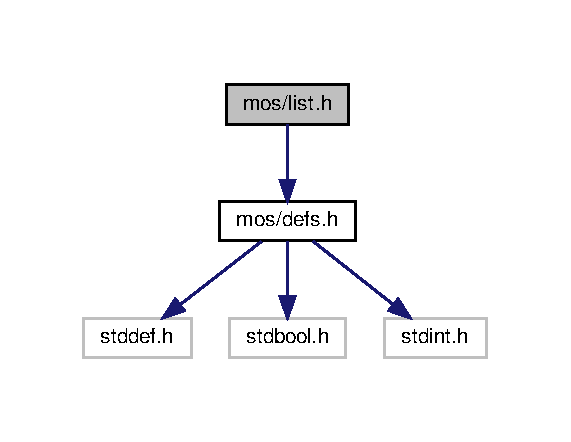
\includegraphics[width=274pt]{list_8h__incl}
\end{center}
\end{figure}
This graph shows which files directly or indirectly include this file\+:\nopagebreak
\begin{figure}[H]
\begin{center}
\leavevmode
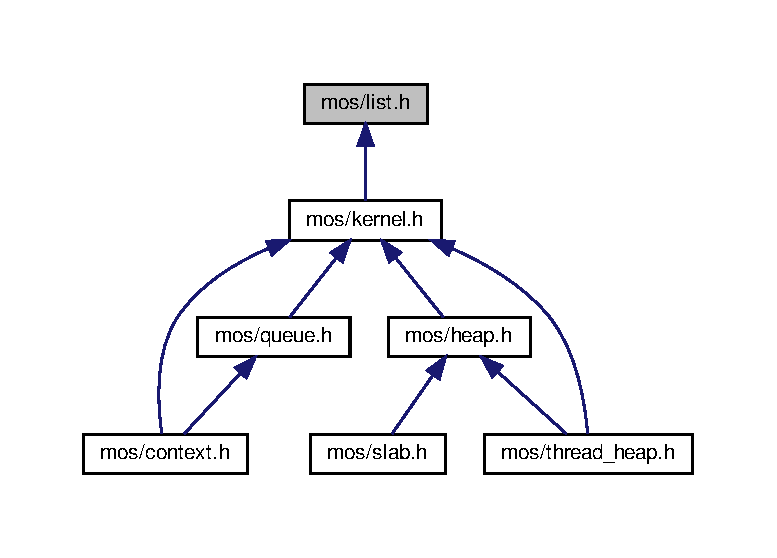
\includegraphics[width=350pt]{list_8h__dep__incl}
\end{center}
\end{figure}
\subsection*{Classes}
\begin{DoxyCompactItemize}
\item 
struct \hyperlink{structMosList}{Mos\+List}
\item 
struct \hyperlink{structMosLinkHet}{Mos\+Link\+Het}
\end{DoxyCompactItemize}
\subsection*{Typedefs}
\begin{DoxyCompactItemize}
\item 
\mbox{\Hypertarget{list_8h_a79af9085d8dead779f159645b6f2c8ae}\label{list_8h_a79af9085d8dead779f159645b6f2c8ae}} 
typedef struct \hyperlink{structMosList}{Mos\+List} {\bfseries Mos\+List}
\item 
\mbox{\Hypertarget{list_8h_a9e353b9a786647e5c95bf65e1c2c371a}\label{list_8h_a9e353b9a786647e5c95bf65e1c2c371a}} 
typedef \hyperlink{structMosList}{Mos\+List} {\bfseries Mos\+Link}
\end{DoxyCompactItemize}
\subsection*{Functions}
\begin{DoxyCompactItemize}
\item 
\mbox{\Hypertarget{list_8h_ab75515acd05b8347d1b307cef3b43269}\label{list_8h_ab75515acd05b8347d1b307cef3b43269}} 
M\+O\+S\+\_\+\+I\+S\+R\+\_\+\+S\+A\+FE void {\bfseries Mos\+Init\+List} (\hyperlink{structMosList}{Mos\+List} $\ast$list)
\item 
\mbox{\Hypertarget{list_8h_adce13e4d021874faf330e17205e3899c}\label{list_8h_adce13e4d021874faf330e17205e3899c}} 
M\+O\+S\+\_\+\+I\+S\+R\+\_\+\+S\+A\+FE void {\bfseries Mos\+Init\+Link\+Het} (\hyperlink{structMosLinkHet}{Mos\+Link\+Het} $\ast$elm, u32 type)
\item 
\mbox{\Hypertarget{list_8h_a790e9df4555980493736c7c16118d448}\label{list_8h_a790e9df4555980493736c7c16118d448}} 
M\+O\+S\+\_\+\+I\+S\+R\+\_\+\+S\+A\+FE void {\bfseries Mos\+Add\+To\+List} (\hyperlink{structMosList}{Mos\+List} $\ast$list, \hyperlink{structMosList}{Mos\+List} $\ast$elm\+\_\+add)
\item 
\mbox{\Hypertarget{list_8h_a7eaf38c11136b2deb64e69ad583acb17}\label{list_8h_a7eaf38c11136b2deb64e69ad583acb17}} 
static M\+O\+S\+\_\+\+I\+N\+L\+I\+NE M\+O\+S\+\_\+\+I\+S\+R\+\_\+\+S\+A\+FE void {\bfseries Mos\+Add\+To\+List\+Before} (\hyperlink{structMosList}{Mos\+List} $\ast$elm\+\_\+exist, \hyperlink{structMosList}{Mos\+List} $\ast$elm\+\_\+add)
\item 
\mbox{\Hypertarget{list_8h_a0e9c6d6a932171c5e7ad1a83b8189840}\label{list_8h_a0e9c6d6a932171c5e7ad1a83b8189840}} 
void M\+O\+S\+\_\+\+I\+S\+R\+\_\+\+S\+A\+FE {\bfseries Mos\+Add\+To\+List\+After} (\hyperlink{structMosList}{Mos\+List} $\ast$elm\+\_\+exist, \hyperlink{structMosList}{Mos\+List} $\ast$elm\+\_\+add)
\item 
\mbox{\Hypertarget{list_8h_a0f719cde66174a0a8723d42b63445a54}\label{list_8h_a0f719cde66174a0a8723d42b63445a54}} 
static M\+O\+S\+\_\+\+I\+N\+L\+I\+NE M\+O\+S\+\_\+\+I\+S\+R\+\_\+\+S\+A\+FE void {\bfseries Mos\+Add\+To\+Front\+Of\+List} (\hyperlink{structMosList}{Mos\+List} $\ast$list, \hyperlink{structMosList}{Mos\+List} $\ast$elm\+\_\+add)
\item 
\mbox{\Hypertarget{list_8h_a6d0593f72884e6283cb82d57316f63f0}\label{list_8h_a6d0593f72884e6283cb82d57316f63f0}} 
void M\+O\+S\+\_\+\+I\+S\+R\+\_\+\+S\+A\+FE {\bfseries Mos\+Remove\+From\+List} (\hyperlink{structMosList}{Mos\+List} $\ast$elm\+\_\+rem)
\item 
\mbox{\Hypertarget{list_8h_a138d8c85dfe867e83c72526ae041e0aa}\label{list_8h_a138d8c85dfe867e83c72526ae041e0aa}} 
void M\+O\+S\+\_\+\+I\+S\+R\+\_\+\+S\+A\+FE {\bfseries Mos\+Move\+To\+End\+Of\+List} (\hyperlink{structMosList}{Mos\+List} $\ast$elm\+\_\+exist, \hyperlink{structMosList}{Mos\+List} $\ast$elm\+\_\+move)
\item 
\mbox{\Hypertarget{list_8h_a348fdf9f9f1770f138172301fe22d943}\label{list_8h_a348fdf9f9f1770f138172301fe22d943}} 
static M\+O\+S\+\_\+\+I\+N\+L\+I\+NE M\+O\+S\+\_\+\+I\+S\+R\+\_\+\+S\+A\+FE bool {\bfseries Mos\+Is\+Last\+Element} (\hyperlink{structMosList}{Mos\+List} $\ast$list, \hyperlink{structMosList}{Mos\+List} $\ast$elm)
\item 
\mbox{\Hypertarget{list_8h_ace5a4e9b055bb46aaed184626d4ff181}\label{list_8h_ace5a4e9b055bb46aaed184626d4ff181}} 
static M\+O\+S\+\_\+\+I\+N\+L\+I\+NE M\+O\+S\+\_\+\+I\+S\+R\+\_\+\+S\+A\+FE bool {\bfseries Mos\+Is\+List\+Empty} (\hyperlink{structMosList}{Mos\+List} $\ast$list)
\item 
\mbox{\Hypertarget{list_8h_a483dbb3d2e225211c1b9e386ae4db93a}\label{list_8h_a483dbb3d2e225211c1b9e386ae4db93a}} 
static M\+O\+S\+\_\+\+I\+N\+L\+I\+NE M\+O\+S\+\_\+\+I\+S\+R\+\_\+\+S\+A\+FE bool {\bfseries Mos\+Is\+On\+List} (\hyperlink{structMosList}{Mos\+List} $\ast$elm)
\end{DoxyCompactItemize}


\subsection{Detailed Description}
Doubly-\/\+Linked Circular Lists. 


\hypertarget{queue_8h}{}\section{mos/queue.h File Reference}
\label{queue_8h}\index{mos/queue.\+h@{mos/queue.\+h}}


M\+OS Message Queues.  


{\ttfamily \#include $<$mos/kernel.\+h$>$}\newline
Include dependency graph for queue.\+h\+:\nopagebreak
\begin{figure}[H]
\begin{center}
\leavevmode
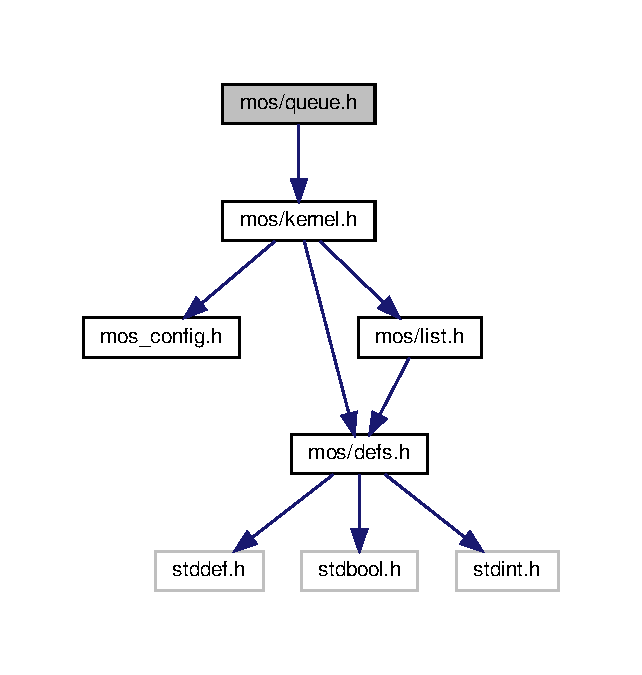
\includegraphics[width=308pt]{queue_8h__incl}
\end{center}
\end{figure}
This graph shows which files directly or indirectly include this file\+:\nopagebreak
\begin{figure}[H]
\begin{center}
\leavevmode
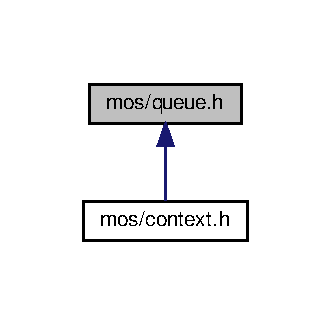
\includegraphics[width=159pt]{queue_8h__dep__incl}
\end{center}
\end{figure}
\subsection*{Classes}
\begin{DoxyCompactItemize}
\item 
struct \hyperlink{structMosQueue}{Mos\+Queue}
\end{DoxyCompactItemize}
\subsection*{Typedefs}
\begin{DoxyCompactItemize}
\item 
\mbox{\Hypertarget{queue_8h_a673c15720267dc3fde85c178e50fb2b7}\label{queue_8h_a673c15720267dc3fde85c178e50fb2b7}} 
typedef struct \hyperlink{structMosQueue}{Mos\+Queue} {\bfseries Mos\+Queue}
\end{DoxyCompactItemize}
\subsection*{Functions}
\begin{DoxyCompactItemize}
\item 
void \hyperlink{queue_8h_a21b09416e970aa60b8665551f80a0c70}{Mos\+Init\+Queue} (\hyperlink{structMosQueue}{Mos\+Queue} $\ast$queue, void $\ast$buf, u32 elm\+\_\+size, u32 num\+\_\+elm)
\item 
void \hyperlink{queue_8h_a77887134ec6780cf27a3c8817cb9b9b2}{Mos\+Send\+To\+Queue} (\hyperlink{structMosQueue}{Mos\+Queue} $\ast$queue, const void $\ast$data)
\item 
M\+O\+S\+\_\+\+I\+S\+R\+\_\+\+S\+A\+FE bool \hyperlink{queue_8h_a155efc41764a85e7df79d69edb28c48a}{Mos\+Try\+Send\+To\+Queue} (\hyperlink{structMosQueue}{Mos\+Queue} $\ast$queue, const void $\ast$data)
\item 
bool \hyperlink{queue_8h_a7b1e996dd4e69ce67a818ab354a5869a}{Mos\+Send\+To\+Queue\+Or\+TO} (\hyperlink{structMosQueue}{Mos\+Queue} $\ast$queue, const void $\ast$data, u32 ticks)
\item 
void \hyperlink{queue_8h_aa6b44f387b77a93b5cddabdf5441ecd3}{Mos\+Receive\+From\+Queue} (\hyperlink{structMosQueue}{Mos\+Queue} $\ast$queue, void $\ast$data)
\item 
M\+O\+S\+\_\+\+I\+S\+R\+\_\+\+S\+A\+FE bool \hyperlink{queue_8h_a6b987366192da0c3842892f8c54d54ed}{Mos\+Try\+Receive\+From\+Queue} (\hyperlink{structMosQueue}{Mos\+Queue} $\ast$queue, void $\ast$data)
\item 
bool \hyperlink{queue_8h_aa4e15ceaba459aaa9cd90b146e8757fe}{Mos\+Receive\+From\+Queue\+Or\+TO} (\hyperlink{structMosQueue}{Mos\+Queue} $\ast$queue, void $\ast$data, u32 ticks)
\item 
void \hyperlink{queue_8h_a7fde9488600e7ce142fa05c138343765}{Mos\+Set\+Multi\+Queue\+Channel} (\hyperlink{structMosQueue}{Mos\+Queue} $\ast$queue, \hyperlink{structMosSem}{Mos\+Signal} $\ast$signal, u16 channel)
\item 
s16 \hyperlink{queue_8h_a600427117ad8ff266897e38c29eb6b6e}{Mos\+Wait\+On\+Multi\+Queue} (\hyperlink{structMosSem}{Mos\+Signal} $\ast$signal, u32 $\ast$flags)
\item 
s16 \hyperlink{queue_8h_ada51cc22b7a1a9f80bf62f56b421fd96}{Mos\+Wait\+On\+Multi\+Queue\+Or\+TO} (\hyperlink{structMosSem}{Mos\+Signal} $\ast$signal, u32 $\ast$flags, u32 ticks)
\item 
M\+O\+S\+\_\+\+I\+N\+L\+I\+NE void \hyperlink{queue_8h_a555b9276bd8e25c45ce33dfd98c1a3a8}{Mos\+Init\+Queue32} (\hyperlink{structMosQueue}{Mos\+Queue} $\ast$queue, u32 $\ast$buf, u32 num\+\_\+elm)
\item 
M\+O\+S\+\_\+\+I\+N\+L\+I\+NE void \hyperlink{queue_8h_a4134e6bd2ff28f2020ad902a9d114375}{Mos\+Send\+To\+Queue32} (\hyperlink{structMosQueue}{Mos\+Queue} $\ast$queue, u32 data)
\item 
M\+O\+S\+\_\+\+I\+S\+R\+\_\+\+S\+A\+FE M\+O\+S\+\_\+\+I\+N\+L\+I\+NE bool \hyperlink{queue_8h_a8c8f70086a55715acb5a21924e4a6a9b}{Mos\+Try\+Send\+To\+Queue32} (\hyperlink{structMosQueue}{Mos\+Queue} $\ast$queue, u32 data)
\item 
M\+O\+S\+\_\+\+I\+N\+L\+I\+NE bool \hyperlink{queue_8h_a10b2e3d921c51986ed3a28ba778801db}{Mos\+Send\+To\+Queue32\+Or\+TO} (\hyperlink{structMosQueue}{Mos\+Queue} $\ast$queue, u32 data, u32 ticks)
\item 
M\+O\+S\+\_\+\+I\+N\+L\+I\+NE u32 \hyperlink{queue_8h_a07ed4eef6fe0d0f0761758ef3f7308c1}{Mos\+Receive\+From\+Queue32} (\hyperlink{structMosQueue}{Mos\+Queue} $\ast$queue)
\item 
M\+O\+S\+\_\+\+I\+S\+R\+\_\+\+S\+A\+FE M\+O\+S\+\_\+\+I\+N\+L\+I\+NE bool \hyperlink{queue_8h_acd6b6023a7fffc3e4b897f2caf1aae13}{Mos\+Try\+Receive\+From\+Queue32} (\hyperlink{structMosQueue}{Mos\+Queue} $\ast$queue, u32 $\ast$data)
\item 
M\+O\+S\+\_\+\+I\+N\+L\+I\+NE bool \hyperlink{queue_8h_ab917b9bc619b544e638b12405bf5bee6}{Mos\+Receive\+From\+Queue32\+Or\+TO} (\hyperlink{structMosQueue}{Mos\+Queue} $\ast$queue, u32 $\ast$data, u32 ticks)
\end{DoxyCompactItemize}


\subsection{Detailed Description}
M\+OS Message Queues. 

Blocking message queues featuring optional priority channels. Allows for multiple writer A\+ND multiple reader contexts. Provides blocking and interrupt-\/safe non-\/blocking modes. 

\subsection{Function Documentation}
\mbox{\Hypertarget{queue_8h_a21b09416e970aa60b8665551f80a0c70}\label{queue_8h_a21b09416e970aa60b8665551f80a0c70}} 
\index{queue.\+h@{queue.\+h}!Mos\+Init\+Queue@{Mos\+Init\+Queue}}
\index{Mos\+Init\+Queue@{Mos\+Init\+Queue}!queue.\+h@{queue.\+h}}
\subsubsection{\texorpdfstring{Mos\+Init\+Queue()}{MosInitQueue()}}
{\footnotesize\ttfamily void Mos\+Init\+Queue (\begin{DoxyParamCaption}\item[{\hyperlink{structMosQueue}{Mos\+Queue} $\ast$}]{queue,  }\item[{void $\ast$}]{buf,  }\item[{u32}]{elm\+\_\+size,  }\item[{u32}]{num\+\_\+elm }\end{DoxyParamCaption})}

Set buffer to use for queue, queue element size and number of elements. Must invoke this function before calling any other queue A\+PI functions. \begin{DoxyNote}{Note}
Element size must be a multiple of 4 (32-\/bits). 
\end{DoxyNote}
\mbox{\Hypertarget{queue_8h_a555b9276bd8e25c45ce33dfd98c1a3a8}\label{queue_8h_a555b9276bd8e25c45ce33dfd98c1a3a8}} 
\index{queue.\+h@{queue.\+h}!Mos\+Init\+Queue32@{Mos\+Init\+Queue32}}
\index{Mos\+Init\+Queue32@{Mos\+Init\+Queue32}!queue.\+h@{queue.\+h}}
\subsubsection{\texorpdfstring{Mos\+Init\+Queue32()}{MosInitQueue32()}}
{\footnotesize\ttfamily M\+O\+S\+\_\+\+I\+N\+L\+I\+NE void Mos\+Init\+Queue32 (\begin{DoxyParamCaption}\item[{\hyperlink{structMosQueue}{Mos\+Queue} $\ast$}]{queue,  }\item[{u32 $\ast$}]{buf,  }\item[{u32}]{num\+\_\+elm }\end{DoxyParamCaption})}

Queues with 32-\/bit data\+Initialize queue for 32-\/bit data \mbox{\Hypertarget{queue_8h_aa6b44f387b77a93b5cddabdf5441ecd3}\label{queue_8h_aa6b44f387b77a93b5cddabdf5441ecd3}} 
\index{queue.\+h@{queue.\+h}!Mos\+Receive\+From\+Queue@{Mos\+Receive\+From\+Queue}}
\index{Mos\+Receive\+From\+Queue@{Mos\+Receive\+From\+Queue}!queue.\+h@{queue.\+h}}
\subsubsection{\texorpdfstring{Mos\+Receive\+From\+Queue()}{MosReceiveFromQueue()}}
{\footnotesize\ttfamily void Mos\+Receive\+From\+Queue (\begin{DoxyParamCaption}\item[{\hyperlink{structMosQueue}{Mos\+Queue} $\ast$}]{queue,  }\item[{void $\ast$}]{data }\end{DoxyParamCaption})}

Receive message from queue, blocking if queue empty. \mbox{\Hypertarget{queue_8h_a07ed4eef6fe0d0f0761758ef3f7308c1}\label{queue_8h_a07ed4eef6fe0d0f0761758ef3f7308c1}} 
\index{queue.\+h@{queue.\+h}!Mos\+Receive\+From\+Queue32@{Mos\+Receive\+From\+Queue32}}
\index{Mos\+Receive\+From\+Queue32@{Mos\+Receive\+From\+Queue32}!queue.\+h@{queue.\+h}}
\subsubsection{\texorpdfstring{Mos\+Receive\+From\+Queue32()}{MosReceiveFromQueue32()}}
{\footnotesize\ttfamily M\+O\+S\+\_\+\+I\+N\+L\+I\+NE u32 Mos\+Receive\+From\+Queue32 (\begin{DoxyParamCaption}\item[{\hyperlink{structMosQueue}{Mos\+Queue} $\ast$}]{queue }\end{DoxyParamCaption})}

Receive message from queue with 32-\/bit data, blocking if queue empty. \mbox{\Hypertarget{queue_8h_ab917b9bc619b544e638b12405bf5bee6}\label{queue_8h_ab917b9bc619b544e638b12405bf5bee6}} 
\index{queue.\+h@{queue.\+h}!Mos\+Receive\+From\+Queue32\+Or\+TO@{Mos\+Receive\+From\+Queue32\+Or\+TO}}
\index{Mos\+Receive\+From\+Queue32\+Or\+TO@{Mos\+Receive\+From\+Queue32\+Or\+TO}!queue.\+h@{queue.\+h}}
\subsubsection{\texorpdfstring{Mos\+Receive\+From\+Queue32\+Or\+T\+O()}{MosReceiveFromQueue32OrTO()}}
{\footnotesize\ttfamily M\+O\+S\+\_\+\+I\+N\+L\+I\+NE bool Mos\+Receive\+From\+Queue32\+Or\+TO (\begin{DoxyParamCaption}\item[{\hyperlink{structMosQueue}{Mos\+Queue} $\ast$}]{queue,  }\item[{u32 $\ast$}]{data,  }\item[{u32}]{ticks }\end{DoxyParamCaption})}

Receive message from queue with 32-\/bit data, blocking if queue empty with timeout. \begin{DoxyReturn}{Returns}
true if message received, false on timeout. 
\end{DoxyReturn}
\mbox{\Hypertarget{queue_8h_aa4e15ceaba459aaa9cd90b146e8757fe}\label{queue_8h_aa4e15ceaba459aaa9cd90b146e8757fe}} 
\index{queue.\+h@{queue.\+h}!Mos\+Receive\+From\+Queue\+Or\+TO@{Mos\+Receive\+From\+Queue\+Or\+TO}}
\index{Mos\+Receive\+From\+Queue\+Or\+TO@{Mos\+Receive\+From\+Queue\+Or\+TO}!queue.\+h@{queue.\+h}}
\subsubsection{\texorpdfstring{Mos\+Receive\+From\+Queue\+Or\+T\+O()}{MosReceiveFromQueueOrTO()}}
{\footnotesize\ttfamily bool Mos\+Receive\+From\+Queue\+Or\+TO (\begin{DoxyParamCaption}\item[{\hyperlink{structMosQueue}{Mos\+Queue} $\ast$}]{queue,  }\item[{void $\ast$}]{data,  }\item[{u32}]{ticks }\end{DoxyParamCaption})}

Receive message from queue, blocking if queue empty with timeout. \begin{DoxyReturn}{Returns}
true if message received, false on timeout. 
\end{DoxyReturn}
\mbox{\Hypertarget{queue_8h_a77887134ec6780cf27a3c8817cb9b9b2}\label{queue_8h_a77887134ec6780cf27a3c8817cb9b9b2}} 
\index{queue.\+h@{queue.\+h}!Mos\+Send\+To\+Queue@{Mos\+Send\+To\+Queue}}
\index{Mos\+Send\+To\+Queue@{Mos\+Send\+To\+Queue}!queue.\+h@{queue.\+h}}
\subsubsection{\texorpdfstring{Mos\+Send\+To\+Queue()}{MosSendToQueue()}}
{\footnotesize\ttfamily void Mos\+Send\+To\+Queue (\begin{DoxyParamCaption}\item[{\hyperlink{structMosQueue}{Mos\+Queue} $\ast$}]{queue,  }\item[{const void $\ast$}]{data }\end{DoxyParamCaption})}

Send message to queue, blocking if queue full. \mbox{\Hypertarget{queue_8h_a4134e6bd2ff28f2020ad902a9d114375}\label{queue_8h_a4134e6bd2ff28f2020ad902a9d114375}} 
\index{queue.\+h@{queue.\+h}!Mos\+Send\+To\+Queue32@{Mos\+Send\+To\+Queue32}}
\index{Mos\+Send\+To\+Queue32@{Mos\+Send\+To\+Queue32}!queue.\+h@{queue.\+h}}
\subsubsection{\texorpdfstring{Mos\+Send\+To\+Queue32()}{MosSendToQueue32()}}
{\footnotesize\ttfamily M\+O\+S\+\_\+\+I\+N\+L\+I\+NE void Mos\+Send\+To\+Queue32 (\begin{DoxyParamCaption}\item[{\hyperlink{structMosQueue}{Mos\+Queue} $\ast$}]{queue,  }\item[{u32}]{data }\end{DoxyParamCaption})}

Send to queue containing 32-\/bit data \mbox{\Hypertarget{queue_8h_a10b2e3d921c51986ed3a28ba778801db}\label{queue_8h_a10b2e3d921c51986ed3a28ba778801db}} 
\index{queue.\+h@{queue.\+h}!Mos\+Send\+To\+Queue32\+Or\+TO@{Mos\+Send\+To\+Queue32\+Or\+TO}}
\index{Mos\+Send\+To\+Queue32\+Or\+TO@{Mos\+Send\+To\+Queue32\+Or\+TO}!queue.\+h@{queue.\+h}}
\subsubsection{\texorpdfstring{Mos\+Send\+To\+Queue32\+Or\+T\+O()}{MosSendToQueue32OrTO()}}
{\footnotesize\ttfamily M\+O\+S\+\_\+\+I\+N\+L\+I\+NE bool Mos\+Send\+To\+Queue32\+Or\+TO (\begin{DoxyParamCaption}\item[{\hyperlink{structMosQueue}{Mos\+Queue} $\ast$}]{queue,  }\item[{u32}]{data,  }\item[{u32}]{ticks }\end{DoxyParamCaption})}

Send message to queue with timeout. \begin{DoxyReturn}{Returns}
true if message sent, false on timeout. 
\end{DoxyReturn}
\mbox{\Hypertarget{queue_8h_a7b1e996dd4e69ce67a818ab354a5869a}\label{queue_8h_a7b1e996dd4e69ce67a818ab354a5869a}} 
\index{queue.\+h@{queue.\+h}!Mos\+Send\+To\+Queue\+Or\+TO@{Mos\+Send\+To\+Queue\+Or\+TO}}
\index{Mos\+Send\+To\+Queue\+Or\+TO@{Mos\+Send\+To\+Queue\+Or\+TO}!queue.\+h@{queue.\+h}}
\subsubsection{\texorpdfstring{Mos\+Send\+To\+Queue\+Or\+T\+O()}{MosSendToQueueOrTO()}}
{\footnotesize\ttfamily bool Mos\+Send\+To\+Queue\+Or\+TO (\begin{DoxyParamCaption}\item[{\hyperlink{structMosQueue}{Mos\+Queue} $\ast$}]{queue,  }\item[{const void $\ast$}]{data,  }\item[{u32}]{ticks }\end{DoxyParamCaption})}

Send message to queue with timeout. \begin{DoxyReturn}{Returns}
true if message sent, false on timeout. 
\end{DoxyReturn}
\mbox{\Hypertarget{queue_8h_a7fde9488600e7ce142fa05c138343765}\label{queue_8h_a7fde9488600e7ce142fa05c138343765}} 
\index{queue.\+h@{queue.\+h}!Mos\+Set\+Multi\+Queue\+Channel@{Mos\+Set\+Multi\+Queue\+Channel}}
\index{Mos\+Set\+Multi\+Queue\+Channel@{Mos\+Set\+Multi\+Queue\+Channel}!queue.\+h@{queue.\+h}}
\subsubsection{\texorpdfstring{Mos\+Set\+Multi\+Queue\+Channel()}{MosSetMultiQueueChannel()}}
{\footnotesize\ttfamily void Mos\+Set\+Multi\+Queue\+Channel (\begin{DoxyParamCaption}\item[{\hyperlink{structMosQueue}{Mos\+Queue} $\ast$}]{queue,  }\item[{\hyperlink{structMosSem}{Mos\+Signal} $\ast$}]{signal,  }\item[{u16}]{channel }\end{DoxyParamCaption})}

Sets signal channel to raise when sending to queue. Lower channel numbers have higher priorities. 
\begin{DoxyParams}{Parameters}
{\em channel} & channel number to set. Signal bit is (1 $<$$<$ channel). \\
\hline
\end{DoxyParams}
\mbox{\Hypertarget{queue_8h_a6b987366192da0c3842892f8c54d54ed}\label{queue_8h_a6b987366192da0c3842892f8c54d54ed}} 
\index{queue.\+h@{queue.\+h}!Mos\+Try\+Receive\+From\+Queue@{Mos\+Try\+Receive\+From\+Queue}}
\index{Mos\+Try\+Receive\+From\+Queue@{Mos\+Try\+Receive\+From\+Queue}!queue.\+h@{queue.\+h}}
\subsubsection{\texorpdfstring{Mos\+Try\+Receive\+From\+Queue()}{MosTryReceiveFromQueue()}}
{\footnotesize\ttfamily M\+O\+S\+\_\+\+I\+S\+R\+\_\+\+S\+A\+FE bool Mos\+Try\+Receive\+From\+Queue (\begin{DoxyParamCaption}\item[{\hyperlink{structMosQueue}{Mos\+Queue} $\ast$}]{queue,  }\item[{void $\ast$}]{data }\end{DoxyParamCaption})}

Attempt to receive message on queue. \begin{DoxyReturn}{Returns}
true if message received, false if empty. 
\end{DoxyReturn}
\mbox{\Hypertarget{queue_8h_acd6b6023a7fffc3e4b897f2caf1aae13}\label{queue_8h_acd6b6023a7fffc3e4b897f2caf1aae13}} 
\index{queue.\+h@{queue.\+h}!Mos\+Try\+Receive\+From\+Queue32@{Mos\+Try\+Receive\+From\+Queue32}}
\index{Mos\+Try\+Receive\+From\+Queue32@{Mos\+Try\+Receive\+From\+Queue32}!queue.\+h@{queue.\+h}}
\subsubsection{\texorpdfstring{Mos\+Try\+Receive\+From\+Queue32()}{MosTryReceiveFromQueue32()}}
{\footnotesize\ttfamily M\+O\+S\+\_\+\+I\+S\+R\+\_\+\+S\+A\+FE M\+O\+S\+\_\+\+I\+N\+L\+I\+NE bool Mos\+Try\+Receive\+From\+Queue32 (\begin{DoxyParamCaption}\item[{\hyperlink{structMosQueue}{Mos\+Queue} $\ast$}]{queue,  }\item[{u32 $\ast$}]{data }\end{DoxyParamCaption})}

Attempt to receive message on queue with 32-\/bit data. \begin{DoxyReturn}{Returns}
true if message received, false if empty. 
\end{DoxyReturn}
\mbox{\Hypertarget{queue_8h_a155efc41764a85e7df79d69edb28c48a}\label{queue_8h_a155efc41764a85e7df79d69edb28c48a}} 
\index{queue.\+h@{queue.\+h}!Mos\+Try\+Send\+To\+Queue@{Mos\+Try\+Send\+To\+Queue}}
\index{Mos\+Try\+Send\+To\+Queue@{Mos\+Try\+Send\+To\+Queue}!queue.\+h@{queue.\+h}}
\subsubsection{\texorpdfstring{Mos\+Try\+Send\+To\+Queue()}{MosTrySendToQueue()}}
{\footnotesize\ttfamily M\+O\+S\+\_\+\+I\+S\+R\+\_\+\+S\+A\+FE bool Mos\+Try\+Send\+To\+Queue (\begin{DoxyParamCaption}\item[{\hyperlink{structMosQueue}{Mos\+Queue} $\ast$}]{queue,  }\item[{const void $\ast$}]{data }\end{DoxyParamCaption})}

Attempt to send message to queue, non-\/blocking. \begin{DoxyReturn}{Returns}
true if message sent. 
\end{DoxyReturn}
\mbox{\Hypertarget{queue_8h_a8c8f70086a55715acb5a21924e4a6a9b}\label{queue_8h_a8c8f70086a55715acb5a21924e4a6a9b}} 
\index{queue.\+h@{queue.\+h}!Mos\+Try\+Send\+To\+Queue32@{Mos\+Try\+Send\+To\+Queue32}}
\index{Mos\+Try\+Send\+To\+Queue32@{Mos\+Try\+Send\+To\+Queue32}!queue.\+h@{queue.\+h}}
\subsubsection{\texorpdfstring{Mos\+Try\+Send\+To\+Queue32()}{MosTrySendToQueue32()}}
{\footnotesize\ttfamily M\+O\+S\+\_\+\+I\+S\+R\+\_\+\+S\+A\+FE M\+O\+S\+\_\+\+I\+N\+L\+I\+NE bool Mos\+Try\+Send\+To\+Queue32 (\begin{DoxyParamCaption}\item[{\hyperlink{structMosQueue}{Mos\+Queue} $\ast$}]{queue,  }\item[{u32}]{data }\end{DoxyParamCaption})}

Send to queue containing 32-\/bit data \mbox{\Hypertarget{queue_8h_a600427117ad8ff266897e38c29eb6b6e}\label{queue_8h_a600427117ad8ff266897e38c29eb6b6e}} 
\index{queue.\+h@{queue.\+h}!Mos\+Wait\+On\+Multi\+Queue@{Mos\+Wait\+On\+Multi\+Queue}}
\index{Mos\+Wait\+On\+Multi\+Queue@{Mos\+Wait\+On\+Multi\+Queue}!queue.\+h@{queue.\+h}}
\subsubsection{\texorpdfstring{Mos\+Wait\+On\+Multi\+Queue()}{MosWaitOnMultiQueue()}}
{\footnotesize\ttfamily s16 Mos\+Wait\+On\+Multi\+Queue (\begin{DoxyParamCaption}\item[{\hyperlink{structMosSem}{Mos\+Signal} $\ast$}]{signal,  }\item[{u32 $\ast$}]{flags }\end{DoxyParamCaption})}

Wait on multiple queues of different priorities. \begin{DoxyReturn}{Returns}
highest priority channel number and updated flags. 
\end{DoxyReturn}
\mbox{\Hypertarget{queue_8h_ada51cc22b7a1a9f80bf62f56b421fd96}\label{queue_8h_ada51cc22b7a1a9f80bf62f56b421fd96}} 
\index{queue.\+h@{queue.\+h}!Mos\+Wait\+On\+Multi\+Queue\+Or\+TO@{Mos\+Wait\+On\+Multi\+Queue\+Or\+TO}}
\index{Mos\+Wait\+On\+Multi\+Queue\+Or\+TO@{Mos\+Wait\+On\+Multi\+Queue\+Or\+TO}!queue.\+h@{queue.\+h}}
\subsubsection{\texorpdfstring{Mos\+Wait\+On\+Multi\+Queue\+Or\+T\+O()}{MosWaitOnMultiQueueOrTO()}}
{\footnotesize\ttfamily s16 Mos\+Wait\+On\+Multi\+Queue\+Or\+TO (\begin{DoxyParamCaption}\item[{\hyperlink{structMosSem}{Mos\+Signal} $\ast$}]{signal,  }\item[{u32 $\ast$}]{flags,  }\item[{u32}]{ticks }\end{DoxyParamCaption})}

Wait on multiple queues with timeout. \begin{DoxyReturn}{Returns}
highest priority channel number and updated flags, -\/1 for timeout. 
\end{DoxyReturn}

\hypertarget{mos__config_8h}{}\section{mos\+\_\+config.\+h File Reference}
\label{mos__config_8h}\index{mos\+\_\+config.\+h@{mos\+\_\+config.\+h}}


M\+OS Configuration File.  


This graph shows which files directly or indirectly include this file\+:\nopagebreak
\begin{figure}[H]
\begin{center}
\leavevmode
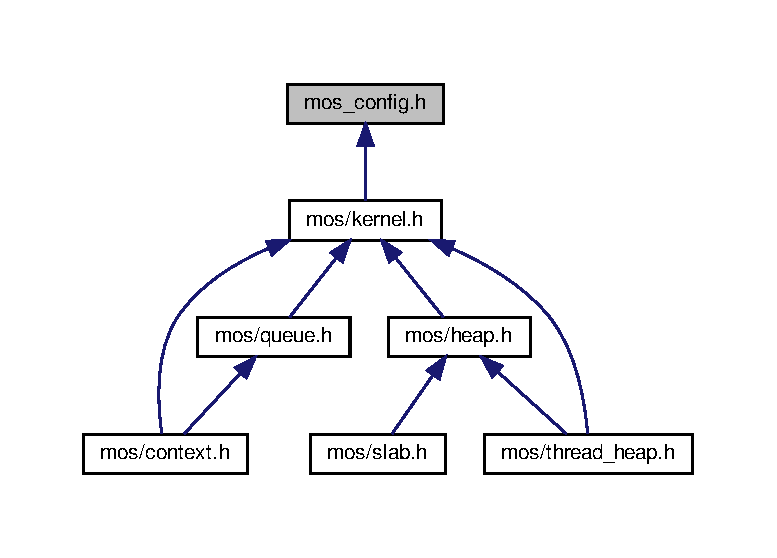
\includegraphics[width=350pt]{mos__config_8h__dep__incl}
\end{center}
\end{figure}
\subsection*{Macros}
\begin{DoxyCompactItemize}
\item 
\#define \hyperlink{mos__config_8h_ad1803148610318396564915f7b05f74a}{M\+O\+S\+\_\+\+M\+A\+X\+\_\+\+T\+H\+R\+E\+A\+D\+\_\+\+P\+R\+I\+O\+R\+I\+T\+I\+ES}~4
\item 
\#define \hyperlink{mos__config_8h_a2db444cd6908c9bfd69826472a49c57c}{M\+O\+S\+\_\+\+M\+I\+C\+R\+O\+\_\+\+S\+E\+C\+\_\+\+P\+E\+R\+\_\+\+T\+I\+CK}~1000
\item 
\#define \hyperlink{mos__config_8h_a01dd2ae0fb6d32216c7d55cc8b7dd11a}{M\+O\+S\+\_\+\+S\+T\+A\+C\+K\+\_\+\+U\+S\+A\+G\+E\+\_\+\+M\+O\+N\+I\+T\+OR}~true
\item 
\#define \hyperlink{mos__config_8h_a6cb750ae6ffedb473238c2976f6c548a}{M\+O\+S\+\_\+\+K\+E\+E\+P\+\_\+\+T\+I\+C\+K\+S\+\_\+\+R\+U\+N\+N\+I\+NG}~false
\item 
\#define \hyperlink{mos__config_8h_a1a0f00b489bf6f3f76448b939a1ce2a7}{M\+O\+S\+\_\+\+E\+N\+A\+B\+L\+E\+\_\+\+E\+V\+E\+N\+TS}~false
\item 
\#define \hyperlink{mos__config_8h_abedfdd335fcdaed1a310e376da4f0afb}{M\+O\+S\+\_\+\+E\+N\+A\+B\+L\+E\+\_\+\+U\+N\+A\+L\+I\+G\+N\+\_\+\+F\+A\+U\+L\+TS}~false
\item 
\#define \hyperlink{mos__config_8h_ac1bbd575a51c5a0705ebb6e6d0a0b9cc}{M\+O\+S\+\_\+\+H\+A\+N\+G\+\_\+\+O\+N\+\_\+\+E\+X\+C\+E\+P\+T\+I\+O\+NS}~false
\end{DoxyCompactItemize}


\subsection{Detailed Description}
M\+OS Configuration File. 

M\+OS is intended to be easy to maintain, so rather than providing tons of options here and cluttering the code with \#ifdefs, instead consider modifying the microkernel itself to suit system requirements. 

\subsection{Macro Definition Documentation}
\mbox{\Hypertarget{mos__config_8h_a1a0f00b489bf6f3f76448b939a1ce2a7}\label{mos__config_8h_a1a0f00b489bf6f3f76448b939a1ce2a7}} 
\index{mos\+\_\+config.\+h@{mos\+\_\+config.\+h}!M\+O\+S\+\_\+\+E\+N\+A\+B\+L\+E\+\_\+\+E\+V\+E\+N\+TS@{M\+O\+S\+\_\+\+E\+N\+A\+B\+L\+E\+\_\+\+E\+V\+E\+N\+TS}}
\index{M\+O\+S\+\_\+\+E\+N\+A\+B\+L\+E\+\_\+\+E\+V\+E\+N\+TS@{M\+O\+S\+\_\+\+E\+N\+A\+B\+L\+E\+\_\+\+E\+V\+E\+N\+TS}!mos\+\_\+config.\+h@{mos\+\_\+config.\+h}}
\subsubsection{\texorpdfstring{M\+O\+S\+\_\+\+E\+N\+A\+B\+L\+E\+\_\+\+E\+V\+E\+N\+TS}{MOS\_ENABLE\_EVENTS}}
{\footnotesize\ttfamily \#define M\+O\+S\+\_\+\+E\+N\+A\+B\+L\+E\+\_\+\+E\+V\+E\+N\+TS~false}

Enable events (required for M\+OS profiling) \mbox{\Hypertarget{mos__config_8h_abedfdd335fcdaed1a310e376da4f0afb}\label{mos__config_8h_abedfdd335fcdaed1a310e376da4f0afb}} 
\index{mos\+\_\+config.\+h@{mos\+\_\+config.\+h}!M\+O\+S\+\_\+\+E\+N\+A\+B\+L\+E\+\_\+\+U\+N\+A\+L\+I\+G\+N\+\_\+\+F\+A\+U\+L\+TS@{M\+O\+S\+\_\+\+E\+N\+A\+B\+L\+E\+\_\+\+U\+N\+A\+L\+I\+G\+N\+\_\+\+F\+A\+U\+L\+TS}}
\index{M\+O\+S\+\_\+\+E\+N\+A\+B\+L\+E\+\_\+\+U\+N\+A\+L\+I\+G\+N\+\_\+\+F\+A\+U\+L\+TS@{M\+O\+S\+\_\+\+E\+N\+A\+B\+L\+E\+\_\+\+U\+N\+A\+L\+I\+G\+N\+\_\+\+F\+A\+U\+L\+TS}!mos\+\_\+config.\+h@{mos\+\_\+config.\+h}}
\subsubsection{\texorpdfstring{M\+O\+S\+\_\+\+E\+N\+A\+B\+L\+E\+\_\+\+U\+N\+A\+L\+I\+G\+N\+\_\+\+F\+A\+U\+L\+TS}{MOS\_ENABLE\_UNALIGN\_FAULTS}}
{\footnotesize\ttfamily \#define M\+O\+S\+\_\+\+E\+N\+A\+B\+L\+E\+\_\+\+U\+N\+A\+L\+I\+G\+N\+\_\+\+F\+A\+U\+L\+TS~false}

Enable \char`\"{}unintentional\char`\"{} alignment faults. Recommend true for small from-\/scratch projects, false for large, pre-\/existing code bases. \mbox{\Hypertarget{mos__config_8h_ac1bbd575a51c5a0705ebb6e6d0a0b9cc}\label{mos__config_8h_ac1bbd575a51c5a0705ebb6e6d0a0b9cc}} 
\index{mos\+\_\+config.\+h@{mos\+\_\+config.\+h}!M\+O\+S\+\_\+\+H\+A\+N\+G\+\_\+\+O\+N\+\_\+\+E\+X\+C\+E\+P\+T\+I\+O\+NS@{M\+O\+S\+\_\+\+H\+A\+N\+G\+\_\+\+O\+N\+\_\+\+E\+X\+C\+E\+P\+T\+I\+O\+NS}}
\index{M\+O\+S\+\_\+\+H\+A\+N\+G\+\_\+\+O\+N\+\_\+\+E\+X\+C\+E\+P\+T\+I\+O\+NS@{M\+O\+S\+\_\+\+H\+A\+N\+G\+\_\+\+O\+N\+\_\+\+E\+X\+C\+E\+P\+T\+I\+O\+NS}!mos\+\_\+config.\+h@{mos\+\_\+config.\+h}}
\subsubsection{\texorpdfstring{M\+O\+S\+\_\+\+H\+A\+N\+G\+\_\+\+O\+N\+\_\+\+E\+X\+C\+E\+P\+T\+I\+O\+NS}{MOS\_HANG\_ON\_EXCEPTIONS}}
{\footnotesize\ttfamily \#define M\+O\+S\+\_\+\+H\+A\+N\+G\+\_\+\+O\+N\+\_\+\+E\+X\+C\+E\+P\+T\+I\+O\+NS~false}

Hang on exceptions. Can be used in systems with watchdog timer reset to reboot \mbox{\Hypertarget{mos__config_8h_a6cb750ae6ffedb473238c2976f6c548a}\label{mos__config_8h_a6cb750ae6ffedb473238c2976f6c548a}} 
\index{mos\+\_\+config.\+h@{mos\+\_\+config.\+h}!M\+O\+S\+\_\+\+K\+E\+E\+P\+\_\+\+T\+I\+C\+K\+S\+\_\+\+R\+U\+N\+N\+I\+NG@{M\+O\+S\+\_\+\+K\+E\+E\+P\+\_\+\+T\+I\+C\+K\+S\+\_\+\+R\+U\+N\+N\+I\+NG}}
\index{M\+O\+S\+\_\+\+K\+E\+E\+P\+\_\+\+T\+I\+C\+K\+S\+\_\+\+R\+U\+N\+N\+I\+NG@{M\+O\+S\+\_\+\+K\+E\+E\+P\+\_\+\+T\+I\+C\+K\+S\+\_\+\+R\+U\+N\+N\+I\+NG}!mos\+\_\+config.\+h@{mos\+\_\+config.\+h}}
\subsubsection{\texorpdfstring{M\+O\+S\+\_\+\+K\+E\+E\+P\+\_\+\+T\+I\+C\+K\+S\+\_\+\+R\+U\+N\+N\+I\+NG}{MOS\_KEEP\_TICKS\_RUNNING}}
{\footnotesize\ttfamily \#define M\+O\+S\+\_\+\+K\+E\+E\+P\+\_\+\+T\+I\+C\+K\+S\+\_\+\+R\+U\+N\+N\+I\+NG~false}

Keep tick interrupt running at slowest rate to maintain time even when there are no timer events scheduled. \mbox{\Hypertarget{mos__config_8h_ad1803148610318396564915f7b05f74a}\label{mos__config_8h_ad1803148610318396564915f7b05f74a}} 
\index{mos\+\_\+config.\+h@{mos\+\_\+config.\+h}!M\+O\+S\+\_\+\+M\+A\+X\+\_\+\+T\+H\+R\+E\+A\+D\+\_\+\+P\+R\+I\+O\+R\+I\+T\+I\+ES@{M\+O\+S\+\_\+\+M\+A\+X\+\_\+\+T\+H\+R\+E\+A\+D\+\_\+\+P\+R\+I\+O\+R\+I\+T\+I\+ES}}
\index{M\+O\+S\+\_\+\+M\+A\+X\+\_\+\+T\+H\+R\+E\+A\+D\+\_\+\+P\+R\+I\+O\+R\+I\+T\+I\+ES@{M\+O\+S\+\_\+\+M\+A\+X\+\_\+\+T\+H\+R\+E\+A\+D\+\_\+\+P\+R\+I\+O\+R\+I\+T\+I\+ES}!mos\+\_\+config.\+h@{mos\+\_\+config.\+h}}
\subsubsection{\texorpdfstring{M\+O\+S\+\_\+\+M\+A\+X\+\_\+\+T\+H\+R\+E\+A\+D\+\_\+\+P\+R\+I\+O\+R\+I\+T\+I\+ES}{MOS\_MAX\_THREAD\_PRIORITIES}}
{\footnotesize\ttfamily \#define M\+O\+S\+\_\+\+M\+A\+X\+\_\+\+T\+H\+R\+E\+A\+D\+\_\+\+P\+R\+I\+O\+R\+I\+T\+I\+ES~4}

\hyperlink{structThread}{Thread} priorities $<$=$>$ \mbox{[}0 ... M\+O\+S\+\_\+\+M\+A\+X\+\_\+\+T\+H\+R\+E\+A\+D\+\_\+\+P\+R\+I\+O\+R\+I\+T\+I\+ES -\/ 1\mbox{]}. The lower the number the higher the priority \mbox{\Hypertarget{mos__config_8h_a2db444cd6908c9bfd69826472a49c57c}\label{mos__config_8h_a2db444cd6908c9bfd69826472a49c57c}} 
\index{mos\+\_\+config.\+h@{mos\+\_\+config.\+h}!M\+O\+S\+\_\+\+M\+I\+C\+R\+O\+\_\+\+S\+E\+C\+\_\+\+P\+E\+R\+\_\+\+T\+I\+CK@{M\+O\+S\+\_\+\+M\+I\+C\+R\+O\+\_\+\+S\+E\+C\+\_\+\+P\+E\+R\+\_\+\+T\+I\+CK}}
\index{M\+O\+S\+\_\+\+M\+I\+C\+R\+O\+\_\+\+S\+E\+C\+\_\+\+P\+E\+R\+\_\+\+T\+I\+CK@{M\+O\+S\+\_\+\+M\+I\+C\+R\+O\+\_\+\+S\+E\+C\+\_\+\+P\+E\+R\+\_\+\+T\+I\+CK}!mos\+\_\+config.\+h@{mos\+\_\+config.\+h}}
\subsubsection{\texorpdfstring{M\+O\+S\+\_\+\+M\+I\+C\+R\+O\+\_\+\+S\+E\+C\+\_\+\+P\+E\+R\+\_\+\+T\+I\+CK}{MOS\_MICRO\_SEC\_PER\_TICK}}
{\footnotesize\ttfamily \#define M\+O\+S\+\_\+\+M\+I\+C\+R\+O\+\_\+\+S\+E\+C\+\_\+\+P\+E\+R\+\_\+\+T\+I\+CK~1000}

Tick rate Interrupt tick rate \mbox{\Hypertarget{mos__config_8h_a01dd2ae0fb6d32216c7d55cc8b7dd11a}\label{mos__config_8h_a01dd2ae0fb6d32216c7d55cc8b7dd11a}} 
\index{mos\+\_\+config.\+h@{mos\+\_\+config.\+h}!M\+O\+S\+\_\+\+S\+T\+A\+C\+K\+\_\+\+U\+S\+A\+G\+E\+\_\+\+M\+O\+N\+I\+T\+OR@{M\+O\+S\+\_\+\+S\+T\+A\+C\+K\+\_\+\+U\+S\+A\+G\+E\+\_\+\+M\+O\+N\+I\+T\+OR}}
\index{M\+O\+S\+\_\+\+S\+T\+A\+C\+K\+\_\+\+U\+S\+A\+G\+E\+\_\+\+M\+O\+N\+I\+T\+OR@{M\+O\+S\+\_\+\+S\+T\+A\+C\+K\+\_\+\+U\+S\+A\+G\+E\+\_\+\+M\+O\+N\+I\+T\+OR}!mos\+\_\+config.\+h@{mos\+\_\+config.\+h}}
\subsubsection{\texorpdfstring{M\+O\+S\+\_\+\+S\+T\+A\+C\+K\+\_\+\+U\+S\+A\+G\+E\+\_\+\+M\+O\+N\+I\+T\+OR}{MOS\_STACK\_USAGE\_MONITOR}}
{\footnotesize\ttfamily \#define M\+O\+S\+\_\+\+S\+T\+A\+C\+K\+\_\+\+U\+S\+A\+G\+E\+\_\+\+M\+O\+N\+I\+T\+OR~true}

Monitor maximum stack usage on context switches 
%--- End generated contents ---

% Index
\backmatter
\newpage
\phantomsection
\clearemptydoublepage
\addcontentsline{toc}{chapter}{Index}
\printindex

\end{document}
